\documentclass[10pt,a4paper]{article}
\usepackage[UTF8,fontset = windows]{ctex}
\setCJKmainfont[BoldFont=黑体,ItalicFont=楷体]{华文中宋}
\usepackage{amssymb,amsmath,amsfonts,amsthm,mathrsfs,dsfont,graphicx}
\usepackage{ifthen,indentfirst,enumerate,color,titletoc}
\usepackage{tikz}
\usepackage{makecell}
\usepackage{longtable}
%\usepackage{mathptmx}

\usetikzlibrary{arrows,calc,intersections,patterns}
\usepackage[bf,small,indentafter,pagestyles]{titlesec}
\usepackage[top=1in, bottom=1in,left=0.8in,right=0.8in]{geometry}
\renewcommand{\baselinestretch}{1.65}
\newtheorem{defi}{定义~}
\newtheorem{eg}{例~}
\newtheorem{ex}{~}
\newtheorem{rem}{注~}
\newtheorem{thm}{定理~}
\newtheorem{coro}{推论~}
\newtheorem{axiom}{公理~}
\newtheorem{prop}{性质~}
\newcommand{\blank}[1]{\underline{\hbox to #1pt{}}}
\newcommand{\bracket}[1]{(\hbox to #1pt{})}
\newcommand{\onech}[4]{\par\begin{tabular}{p{.9\textwidth}}
A.~#1\\
B.~#2\\
C.~#3\\
D.~#4
\end{tabular}}
\newcommand{\twoch}[4]{\par\begin{tabular}{p{.46\textwidth}p{.46\textwidth}}
A.~#1& B.~#2\\
C.~#3& D.~#4
\end{tabular}}
\newcommand{\vartwoch}[4]{\par\begin{tabular}{p{.46\textwidth}p{.46\textwidth}}
(1)~#1& (2)~#2\\
(3)~#3& (4)~#4
\end{tabular}}
\newcommand{\fourch}[4]{\par\begin{tabular}{p{.23\textwidth}p{.23\textwidth}p{.23\textwidth}p{.23\textwidth}}
A.~#1 &B.~#2& C.~#3& D.~#4
\end{tabular}}
\newcommand{\varfourch}[4]{\par\begin{tabular}{p{.23\textwidth}p{.23\textwidth}p{.23\textwidth}p{.23\textwidth}}
(1)~#1 &(2)~#2& (3)~#3& (4)~#4
\end{tabular}}
\begin{document}
\begin{enumerate}[1.]

\item 求函数$y=\dfrac{3x-1}{x+1}$的值域.
\item 求函数$y=\dfrac{4x+3}{2x-1}$的值域.
\item 求函数$y=\dfrac{x^2-1}{x^2+2}$的值域.
\item 求函数$y=\dfrac{x^2-x+1}{2x^2-2x+3}$的值域.
\item 求函数$y=\dfrac{x^2+4x+3}{x^2+x-6}$的值域.
\item 若实数$x,y$满足$x^2+4y^2=4x$, 求$S=x^2+y^2$的值域.
\item 已知函数$y=f(x)=x^2+ax+3$在区间$x\in [-1,1]$上的最小值为$-3$, 求实数$a$的值.
\item 求函数$y=3x^2-12x+18\sqrt {4x-x^2}-23$的值域.
\item 求函数$y=|x-2|-|x+1|$的值域.
\item 若$f(x-1)=2x^2+1$, 求$f(x)$.
\item 已知定义域为$\mathbf{R}$的函数$f(x)$满足:
\textcircled{1} $f(x+y)=f(x)\cdot f(y)$对任何实数$x,y$都成立;
\textcircled{2} 存在实数$x_1,x_2$, 使$f(x_1)\ne f(x_2)$.
求证:\\
(1) $f(0)=1$;\\
(2) $f(x)>0$.
\item 设映射$f:X\to Y$, 其中$X,Y$是非空集合, 则下列语句中正确的是\bracket{20}.
\twoch{$Y$中每一个元素必有原像}{$Y$中的各元素只能有一个原像}{$X$中的不同元素在$Y$中的像也不同}{$Y$中至少存在一个元素, 它有原像}
\item 集合$M=\{a,b,c\}$与$P=\{x,y,z\}$之间建立起四种对应关系(如图), 则下列结论中正确的是\bracket{20}.
\begin{center}
    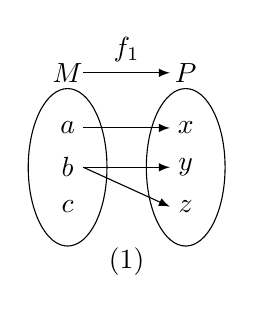
\begin{tikzpicture}[>=latex]
        \draw (0,0) ellipse (0.5 and 1);
        \draw (0,0.5) node {$a$} (0,0) node {$b$} (0,-0.5) node {$c$};
        \draw (1.5,0) ellipse (0.5 and 1);
        \draw (1.5,0.5) node {$x$} (1.5,0) node {$y$} (1.5,-0.5) node {$z$};
        \draw [->] (0.2,0.5) -- (1.3,0.5);
        \draw [->] (0.2,0) -- (1.3,0);
        \draw [->] (0.2,0) -- (1.3,-0.5);
        \draw [->] (0.2,1.2) -- (1.3,1.2);
        \draw (0,1.2) node {$M$} (1.5,1.2) node{$P$};
        \draw (0.75,1.5) node {$f_1$} (0.75,-1.2) node {(1)};
    \end{tikzpicture}
    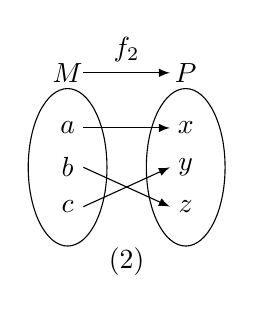
\begin{tikzpicture}[>=latex]
      \draw (0,0) ellipse (0.5 and 1);
      \draw (0,0.5) node {$a$} (0,0) node {$b$} (0,-0.5) node {$c$};
      \draw (1.5,0) ellipse (0.5 and 1);
      \draw (1.5,0.5) node {$x$} (1.5,0) node {$y$} (1.5,-0.5) node {$z$};
      \draw [->] (0.2,0.5) -- (1.3,0.5);
      \draw [->] (0.2,0) -- (1.3,-0.5);
      \draw [->] (0.2,-0.5) -- (1.3,0);
      \draw [->] (0.2,1.2) -- (1.3,1.2);
      \draw (0,1.2) node {$M$} (1.5,1.2) node{$P$};
      \draw (0.75,1.5) node {$f_2$} (0.75,-1.2) node {(2)};
  \end{tikzpicture}
  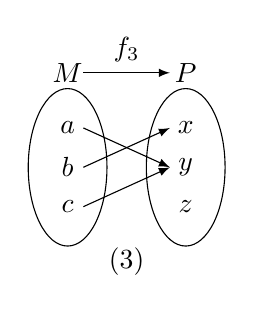
\begin{tikzpicture}[>=latex]
    \draw (0,0) ellipse (0.5 and 1);
    \draw (0,0.5) node {$a$} (0,0) node {$b$} (0,-0.5) node {$c$};
    \draw (1.5,0) ellipse (0.5 and 1);
    \draw (1.5,0.5) node {$x$} (1.5,0) node {$y$} (1.5,-0.5) node {$z$};
    \draw [->] (0.2,0.5) -- (1.3,0);
    \draw [->] (0.2,0) -- (1.3,0.5);
    \draw [->] (0.2,-0.5) -- (1.3,0);
    \draw [->] (0.2,1.2) -- (1.3,1.2);
    \draw (0,1.2) node {$M$} (1.5,1.2) node{$P$};
    \draw (0.75,1.5) node {$f_3$} (0.75,-1.2) node {(3)};
\end{tikzpicture}
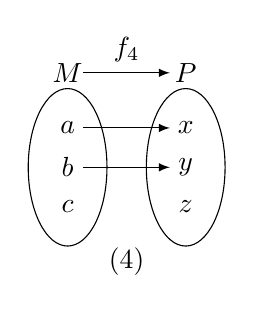
\begin{tikzpicture}[>=latex]
  \draw (0,0) ellipse (0.5 and 1);
  \draw (0,0.5) node {$a$} (0,0) node {$b$} (0,-0.5) node {$c$};
  \draw (1.5,0) ellipse (0.5 and 1);
  \draw (1.5,0.5) node {$x$} (1.5,0) node {$y$} (1.5,-0.5) node {$z$};
  \draw [->] (0.2,0.5) -- (1.3,0.5);
  \draw [->] (0.2,0) -- (1.3,0);
  \draw [->] (0.2,1.2) -- (1.3,1.2);
  \draw (0,1.2) node {$M$} (1.5,1.2) node{$P$};
  \draw (0.75,1.5) node {$f_4$} (0.75,-1.2) node {(4)};
\end{tikzpicture}
\end{center}
\twoch{只有$f_2,f_3$是从$M$到$P$的映射}{只有$f_2,f_4$是从$M$到$P$的映射}{只有$f_3,f_4$是从$M$到$P$的映射}{$f_1,f_2,f_3,f_4$都是从$M$到$P$的映射}
\item 设$(x,y)$在映射$f$下的像是$(\dfrac{x+y}2,\dfrac{x-y}2)$, 则在$f$下$(-5,2)$的原像是\bracket{20}.
\fourch{$(-10,4)$}{$(-3,-7)$}{$(-6,-4)$}{$(-\dfrac 32,-\dfrac 72)$}
\item 在给定的映射$f:(x,y)\mapsto (2x+y,xy)$($x,y\in \mathbf{R}$)下, 点$(\dfrac 16,-\dfrac 16)$的原像是\bracket{20}.
\fourch{$(\dfrac 16,-\dfrac 1{36})$}{$(\dfrac 13,-\dfrac 12)$或$(-\dfrac 14,\dfrac 23)$}{$(\dfrac 1{36},-\dfrac 16)$}{$(\dfrac 12,-\dfrac 13)$或$(-\dfrac 23,\dfrac 14)$}
\item 已知集合$M=\{x|0\le x\le 6\}$, $P=\{0\le y\le 3\}$, 则下列对应关系中, 不能作为从$M$到$P$的映射的是\bracket{20}.
\fourch{$f:x\mapsto y=\dfrac 12x$}{$f:x\mapsto y=\dfrac 13x$}{$f:x\mapsto y=x$}{$f:x\mapsto y=\dfrac 16x$}
\item 设$M=\mathbf{R}$, 从$M$到$P$的映射$f:x\mapsto y=\dfrac 1{x^2+1}$, 则像集$P$为\bracket{20}.
\fourch{$\{y|y\in \mathbf{R}\}$}{$\{y|y\in \mathbf{R}\}$}{$\{y|0\le y\le 2\}$}{$\{y|0<y\le 1\}$}
\item 若映射$f:A\to B$的像集是$Y$, 原像的集合是$X$, 则$X$与$A$的关系是\blank{50}, $Y$和$B$的关系是\blank{50}.
\item 若$(x,y)$在映射$f$下的像是$(2x-y,x+2y)$, 则$(-1,2)$在$f$下的原像是\blank{50}.
\item 已知$(a,b)$在映射$f$的像是$(a-b,ab)$, 则$(2,3)$的原像是\blank{50}.
\item 已知$f:x\mapsto y=x^2$是从集合$\mathbf{R}$到集合$M=\{x|x\ge 0\}$的一个映射, 则$M$中的元素$1$在$\mathbf{R}$中的原像是\blank{50}, $M$中的元素$t$($t>0$)在$\mathbf{R}$中的原像是\blank{50}.
\item 从集合$\{a\}$到$\{b,c\}$的不同映射有\blank{50}个.
\item 从集合$\{1,2\}$到$\{5,6\}$的不同映射有\blank{50}个.
\item 已知集合$A=\mathbf{Z}$, $B=\{x|x=2n+1, \ n\in \mathbf{Z}\}$, $C=\mathbf{R}$, 且从$A$到$B$的映射是$x\mapsto 2x-1$, 从$B$到$C$的映射是$x\mapsto \dfrac 1{3x+1}$, 则从$A$到$C$的映射是\blank{50}.
\item $f$是集合$X=\{a,b,c\}$到集合$Y=\{d,e\}$的一个映射, 则满足映射条件的``$f$''共有\bracket{20}.
\fourch{$5$个}{$6$个}{$7$个}{$8$个}
\item 若$f:y=3x+1$是从集合$A=\{1,2,3,k\}$到集合$B=\{4,7,a^4,a^2+3a\}$的一个映射, 求自然数$a,k$的值及集合$A,B$.
\item 函数$f(x)=\dfrac{\sqrt{x^2-5x+6}}{x-2}$的定义域是\bracket{20}.
\fourch{$\{x|2<x<3\}$}{$\{x|x<2x>3\}$}{$\{x|x\le 2x\ge 3\}$}{$\{x|x<2\text{或}x\ge 3\}$}
\item 若函数$f(x)$的定义域是$[-1,1]$, 则函数$f(x+1)$的定义域是\bracket{20}.
\fourch{$[-1,1]$}{$[0,2]$}{$[-2,0]$}{$[0,1]$}
\item 在\textcircled{1} $y=x$与$y=\sqrt {x^2}$; \textcircled{2} $y=\sqrt {x^2}$与$y=(\sqrt x)^2$; \textcircled{3} $y=|x|$与$y=\dfrac{x^2}x$; \textcircled{4} $y=|x|$与$y=\sqrt {x^2}$; \textcircled{5} $y=x^0$与$y=1$这五组函数中, 表示同一函数的组数是\bracket{20}.
\fourch{$0$}{$1$}{$2$}{$3$}
\item 函数$y=-x^2-2x+3(-5\le x\le 0)$的值域是\bracket{20}.
\fourch{$(-\infty ,4]$}{$[3,12]$}{$[-12,4]$}{$[4,12]$}
\item 已知镭经过$100$年后剩下原来质量的$95.76\%$, 若质量为$l$克的镭经过$x$年后的剩余质量为$y$克, 则$y$与$x$之间的解析式是\bracket{20}.
\fourch{$y=(\dfrac{0.9576}{100})^x$}{$y=(0.9576)^{100x}$}{$y=(0.9576)^{\frac x{100}}$}{$y=1-(1-0.9576)^{\frac x{100}}$}
\item 函数$y=x+\dfrac{|x|}x$的图像是\bracket{20}.
\fourch{\begin{tikzpicture}[scale = 0.7,>=latex]
\draw [->] (-2,0) -- (2,0) node [below] {$x$};
\draw [->] (0,-2) -- (0,2) node [left] {$y$};
\draw (0,0) node [below right] {$O$};
\draw (-1,0) node [below] {$-1$} (0,1) node [right] {$1$};
\draw (-2,-1) -- (1,2);
\filldraw [white] (0,1) circle (0.05);
\draw (0,1) circle (0.05);
\end{tikzpicture}}{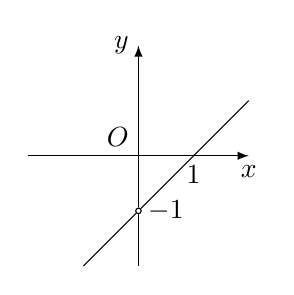
\begin{tikzpicture}[scale = 0.7,>=latex]
\draw [->] (-2,0) -- (2,0) node [below] {$x$};
\draw [->] (0,-2) -- (0,2) node [left] {$y$};
\draw (0,0) node [above left] {$O$};
\draw (1,0) node [below] {$1$} (0,-1) node [right] {$-1$};
\draw (-1,-2) -- (2,1);
\filldraw [white] (0,-1) circle (0.05);
\draw (0,-1) circle (0.05);
\end{tikzpicture}}{\begin{tikzpicture}[scale = 0.7,>=latex]
\draw [->] (-2,0) -- (2,0) node [below] {$x$};
\draw [->] (0,-2) -- (0,2) node [left] {$y$};
\draw (0,0) node [below right] {$O$};
\draw (1,0.1) -- (1,0) node [below] {$1$} (0,-1) node [right] {$-1$} (0,1) node [right] {$1$} (-1,0.1) -- (-1,0) node [below] {$-1$};
\draw (-1,-2) -- (0,-1) (0,1) -- (1,2);
\filldraw [white] (0,-1) circle (0.05);
\draw (0,-1) circle (0.05);
\filldraw [white] (0,1) circle (0.05);
\draw (0,1) circle (0.05);
\end{tikzpicture}}{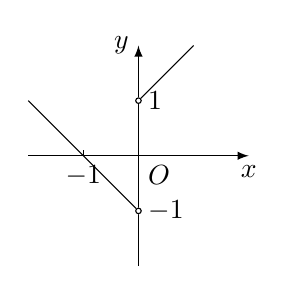
\begin{tikzpicture}[scale = 0.7,>=latex]
\draw [->] (-2,0) -- (2,0) node [below] {$x$};
\draw [->] (0,-2) -- (0,2) node [left] {$y$};
\draw (0,0) node [below right] {$O$};
\draw (0,-1) node [right] {$-1$} (0,1) node [right] {$1$} (-1,0.1) -- (-1,0) node [below] {$-1$};
\draw (-2,1) -- (0,-1) (0,1) -- (1,2);
\filldraw [white] (0,-1) circle (0.05);
\draw (0,-1) circle (0.05);
\filldraw [white] (0,1) circle (0.05);
\draw (0,1) circle (0.05);
\end{tikzpicture}}
\item 函数$y=\sqrt {1-x^2}+\sqrt {x+1}$的定义域为\blank{50}.
\item 函数$y=\dfrac 1{\sqrt {2x^2+3}}$的定义域为\blank{50}.
\item 函数$y=\dfrac{x+5}{3x^2-2x-1}$的定义域为\blank{50}.
\item 函数$y=\sqrt {6x-x^2-9}$的定义域为\blank{50}.
\item 函数$y=\sqrt {4-x^2}+\dfrac 1{|x|-1}$的定义域为\blank{50}.
\item 函数$y=\dfrac{x^3-1}{x+|x|}$的定义域为\blank{50}.
\item 函数$y=\dfrac 1{|x|-x^2}$的定义域为\blank{50}.
\item 函数$y=\sqrt {1-(\dfrac{x-1}{x+1})^2}$的定义域为\blank{50}.
\item 函数$y=\dfrac{\sqrt {x^2-2x-15}}{|x+3|-8}$的定义域为\blank{50}.
\item 函数$y=1-\dfrac 1{x+2}$的值域为\blank{50}.
\item 函数$y=\dfrac 3{2x}$的值域为\blank{50}.
\item 函数$y=\dfrac{x+3}{x-3}$的值域为\blank{50}.
\item 函数$y=\dfrac{5x+3}{x-3}$的值域为\blank{50}.
\item 函数$y=4+\sqrt {2x+1}$的值域为\blank{50}.
\item 函数$y=\sqrt {x-\dfrac 12x^2}$的值域为\blank{50}.
\item 函数$y=\sqrt {-x^2+x+2}$的值域为\blank{50}.
\item 函数$y=\dfrac{2x^2+2x+3}{x^2+x+1}$的值域为\blank{50}.
\item 若函数$f(x)$满足$f(2x)=(1-\sqrt 2x)(1+\sqrt 2x)$, 则$f(x)=$\blank{50}.
\item 若函数$f(x)$满足$f(\sqrt x+1)=x+2\sqrt x$, 则当$x\ge 1$时, $f(x)=$\blank{50}.
\item 若函数$f(x)$满足$f(\dfrac 1x)=\dfrac x{1-x^2}$, 则当$x\ne 0$时, $f(x)=$\blank{50}.
\item 若函数$f(x)=2x+1$, $g(x)=x^2+2$, 满足$f(g(x))=g(f(x))$, 则$x=$\blank{50}.
\item 若函数$f(x)$满足$f(x+1)=2x^2+1$, 则$f(x-1)=$\blank{50}.
\item 若一次函数$f(x)$满足$f(f(x))=1+2x$, 则$f(x)=$\blank{50}.
\item 若$f(x^2-x)=x^4-2x^3+x^2+1$, 则当$x\ge -\dfrac 14$时, $f(f(x))=$\blank{50}.
\item 函数$f(x)=\dfrac x{\sqrt {1+x^2}}$, 则$f(f(x))=$\blank{50}, $f(f(f(x)))=$\blank{50}.
\item 若$-b<a<0$, 且函数$d(x)$的定义域是$[a,b]$, 则函数$F(x)=f(x)+f(-x)$的定义域是\bracket{20}.
\fourch{$[a,b]$}{$[-b,-a]$}{$[-b,b]$}{$[a,-a]$}
\item 若$f(x)$的定义域是$[ 0,1 ]$, 且$f(x+m)+f(x-m)$的定义域是$\varnothing$, 则正数$m$的取值范围是\bracket{20}.
\fourch{$0<m<1$}{$0<m\le \dfrac 12$}{$0<m<\dfrac 12$}{$m>\dfrac 12$}
\item 函数$y=\dfrac{x^2-1}{x^2+1}$的值域是\bracket{20}.
\fourch{$(-1,1)$}{$[-1,1]$}{$[-1,1)$}{$(-1,1]$}
\item 若$2x^2-3x\le 0$, 则函数$f(x)=x^2+x+1$\bracket{20}.
\twoch{有最小值$\dfrac 34$, 但无最大值}{有最小值$\dfrac 34$, 有最大值1}{有最小值1有最大值$\dfrac{19}4$}{既无最小值, 也无最大值}
\item 函数$f(x)=|1-x|-|x-3|(x\in \mathbf{R})$的值域是\bracket{20}.
\fourch{$[-2,2]$}{$[-1,3]$}{$[-3,1]$}{$[0,4]$}
\item 若函数$f(x)$的定义域是$[0,1]$, 分别求函数$f(1-2x)$和$f(x+a)$($a>0$)的定义域.
\item 若函数$f(x+1)$的定义域是$[-2,3)$, 求函数$f(\dfrac 1x+2)$的定义域.
\item 求函数$y=\dfrac{2x}{x^2+x+1}$的值域.
\item 求函数$y=\dfrac{x^2+x-1}{x^2+x+1}$的值域.
\item 求函数$y=\dfrac{x^2-1}{x^2-5x+4}$的值域.
\item 若实数$x,y$满足$3x^2+2y^2=6x$, 分别求$x$与$x^2+y^2$的取值范围.
\item 若实数$x,y$满足$x^2+y^2=2x$, 求$x^2-y^2$的取值范围.
\item 求函数$y=3x-2+\sqrt {3-2x}$的值域.
\item 求函数$y=2x+\sqrt {2x-1}$的值域.
\item 求函数$y=(x-1)(x-2)(x-3)(x-4)+15$的值域.
\item 已知函数$f(x)=x^2-2x+3$在$[0,m]$上有最大值$3$, 最小值$2$, 求正数$m$的取值范围.
\item 已知函数$y=x^2+mx-1$在区间$[0,3]$上有最小值$-2$, 求实数$m$的值.
\item 当$x\ge 0$时, 求函数$f(x)=x^2+2ax$的最小值.
\item 已知函数$f(x)=\dfrac{ax}{2x+3}$($x\ne -\dfrac 32$)满足$f(f(x))=x$, 求实数$a$的值.
\item 已知$f(x)$是二次函数, 且满足$f(2x)+f(3x+1)=13x^2+6x-1$, 求$f(x)$的表达式.
\item 已知函数$f(x)$的定义域是一切非零实数, 且满足$3f(x)+2f(\dfrac 1x)=4x$, 求, $f(x)$的表达式.
\item 作出函数$y=1+\dfrac{|x|}x$的图像.
\item 作出函数$y=x-|1-x|$的图像.
\item 作出函数$y=|x^2-4x+3|$的图像.
\item 作出函数$y=\dfrac{x^3+x}{|x|}$的图像.
\item 作出函数$y=\dfrac{(x+\dfrac 12)}{|x|-x}^0$的图像.
\item 已知$f(x)=-x^2+2x+3$, 画出函数$y=\dfrac 12[f(x)+|f(x)|]$的图像.
\item 已知$f(x)=|x|$, $x\in [-1,1]$, 作出函数$y=f(x+1)+1$的图像.
\item 将进货单价为$40$元的商品按每件$50$元出售时, 每月能卖出$500$个, 已知这批商品在销售单价的基础上每涨价$1$元, 其月销售数就减少$10$个, 为了每月赚取最大利润, 销售单价应定为多少?
\item 飞机飞行$1$小时的耗费由两部分组成: 固定部分$4900$元, 变动部分$P$与飞机飞行速度$v$(千米/时)的函数关系是$P=0.01v^2$. 已知甲、乙两地相距为一常数$a$(千米), 试写出飞机从甲地飞到乙地的总耗费$y$与飞机速度$v$的函数关系式, 并写出耗费最小时飞机的飞行速度.
\item 求证: 函数$f(x)=x^3$在$x\in \mathbf{R}$上是增函数.
\item 已知奇函数$y=f(x)$在$x<0$时是减函数, 求证: $y=f(x)$在$x>0$时也是减函数.
\item 已知$f(x)$是奇函数, 且当$x>0$时$f(x)=x(1-x)$, 求$f(x)$在$x<0$时的表达式.
\item 已知函数$y=f(x)$满足$f(x)=f(4-x)$($x\in \mathbf{R}$), 且$f(x)$在$x>2$时为增函数, 记$a=f(\dfrac 35)$, $b=f(\dfrac 65)$, $c=f(4)$, 则$a,b,c$之间的大小关系是\bracket{20}.
\fourch{$c>a>b$}{$c>b>a$}{$b>a>c$}{$a>c>d$}
\item 画出函数$y=x^2-2|x|-1$的图像.
\item 求函数$y=\dfrac{x-2}{2x+1}$的值域.
\item 已知函数$f(x)=(x-1)^2$($x\le 1$), 又$f(x)$和$\varphi (x)$的图像关于直线$y=x$对称, 求$\varphi (x)$的表达式.
\item 求实数$m$的范围, 使关于$x$的方程$x^2+2(m-1)x+2m+6=0$:\\
(1) 有两个实数根, 且一个比$2$大, 另一个比$2$小;\\
(2) 有两个实数根, 且都比$1$大;\\
(3) 有两个实数根$\alpha ,\beta$, 且满足$0<\alpha <1<\beta <4$;\\
(4) 至少有一个正根.
\item 就参数$m$讨论方程$x^2-2|x|-m=0$的解的情况.
\item 下列记数中, 符合科学记数法的是\bracket{20}.
\fourch{$35.6\times 10^{-25}$}{$0.356\times 10^{-23}$}{$3.56\times 10^{-24}$}{$356\times 10^{-26}$}
\item 计算$3^{-1}\times 2^{-2}\div 4^{-2}$的结果是\bracket{20}.
\fourch{$\dfrac 1{192}$}{$\dfrac 43$}{$\dfrac 1{12}$}{$-\dfrac 43$}
\item 下列各式中, 正确的是\bracket{20}.
\fourch{$(-1)^0=-1$}{$(-1)^{-1}=1$}{$3a^{-2}=\dfrac 1{3a^2}$}{$(-x)^5\div (-x)^3=x^2$}
\item 下列各式中, 计算正确的是\bracket{20}.
\twoch{$(-0.125)\div (-0.5)^{-3}=1$}{$10^{-4}(\sqrt 5)^0=-10000$}{$(\dfrac 13)^0\div 3^{-1}=3$}{$(\sqrt 3-\sqrt 2)^0-(\sqrt 3)^2-(-\sqrt 2)^2=1-3+2=0$}
\item 化简$\dfrac 13x\sqrt {9x}-x^2\sqrt {\dfrac 1x}$的结果是\bracket{20}.
\fourch{$\sqrt x$}{$x(1-x^2)\sqrt x$}{$x^2(1-x\sqrt x)$}{0}
\item 化简$\dfrac{a^{-2}-b^{-2}}{a^2-b^2}$的结果是\bracket{20}.
\fourch{-1}{$-\dfrac 1{a^2b^2}$}{$a^{-1}+b^{-1}$}{$\dfrac 1{a^2b^2}$}
\item 已知$x=1-2^s$, $y=1-2^{-s}$, 则$y$等于\bracket{20}.
\fourch{$\dfrac{x-1}x$}{$\dfrac{2-x}{1-x}$}{$\dfrac x{x-1}$}{$\dfrac{x-2}{x-1}$}
\item 计算$\sqrt {(3-\pi)^2}$的结果是\bracket{20}.
\fourch{$3-\pi$}{$\pi -3$}{$\pi +3$}{$-\pi -3$}
\item 若$(\sqrt [n]{-3})^n$有意义, 则$n$一定是\bracket{20}.
\fourch{正偶数}{自然数}{正奇数}{整数}
\item 已知$n\in \mathbf{N}$, 在\textcircled{1} $\sqrt [4]{(-4)^{2n}}$; \textcircled{2} $\sqrt [4]{(-4)^{2n+1}}$; \textcircled{3} $\sqrt [5]{-x^2}$; \textcircled{4} $\sqrt [5]{-x^2}$这四个式子中, 有意义的\bracket{20}.
\fourch{是\textcircled{1}\textcircled{2}\textcircled{3}\textcircled{4} }{只有\textcircled{3}\textcircled{4}}{只有\textcircled{1}\textcircled{3}\textcircled{4}}{只有\textcircled{4}}
\item 若$\sqrt [4]{4a^2-4a+1}=\sqrt [3]{1-2a}$, 则实数$a$的取值范围是\bracket{20}.
\fourch{$a<2$}{$a=\dfrac 12$或0}{$a>\dfrac 12$}{$R$}
\item 在\textcircled{1} $0^{-1}$; \textcircled{2} $0^{-\frac 12}$; \textcircled{3} $0^0$; \textcircled{4} $0^{0.2}$这四个式子中, 有意义的个数是\bracket{20}.
\fourch{$0$}{$1$}{$2$}{$3$}
\item 下列各式中正确的是\bracket{20}.
\fourch{$-4^0=1$}{$(5^{-\frac 12})^2=5$}{$(-3^{m-n})^2=9^{m-n}$}{$(-2)^{-1}=\dfrac 12$}
\item 计算$[ (-3)^2 ]^{\frac 12}-(-10)^0$的值等于\bracket{20}.
\fourch{$-2$}{$2$}{$-4$}{$4$}
\item 下列计算中正确的是\bracket{20}.
\fourch{$a^{\frac 83}\cdot a^{\frac 38}=a$}{$a^{\frac 83}\cdot a^{-\frac 83}=0$}{$a^{\frac 83}\div a^{\frac 13}=a^8$}{$a^{\frac 12}\div a^{\frac 13}=a^{\frac 16}$}
\item 下列计算中正确的是\bracket{20}.
\fourch{$a^{\frac 34}\cdot a^{\frac 43}=a$}{$a^{\frac 34}\div a^{\frac 34}=a$}{$a^{-4}\div a^4=0$}{$(a^{\frac 34})^{\frac 43}=a$}
\item 化简$(a^{\frac 23}b^{\frac 12})(-3a^{\frac 12}b^{\frac 13})\div (\frac 13a^{\frac 16}b^{\frac 56})$的结果是\bracket{20}.
\fourch{$6a$}{$-a$}{$-9a$}{$9a$}
\item 将$\sqrt [3]{-2\sqrt 2}$化成不含根号的式子是\bracket{20}.
\fourch{$-2^{\frac 12}$}{$-2^{-\frac 12}$}{$-2^{\frac 13}$}{$-2^{\frac 23}$}
\item 将$(a^{\frac 1n}+b^{\frac 1n})^{\frac 13}$表示成根式的形式是\bracket{20}.
\fourch{$\sqrt [3]{a^{\frac 1n}+b^{\frac 1n}}$}{$(\sqrt[n]a+\sqrt[n]b)^{\frac 13}$}{$\sqrt [3]{\sqrt[n]a+\sqrt[n]b}$}{$(\sqrt[n]a+\sqrt[n]b)^3$}
\item 计算: $\sqrt {12}-\sqrt 3\div (2+\sqrt 3)=$\blank{50}.
\item 计算: $(\sqrt {12}-\sqrt {\dfrac 12}-2\sqrt {\dfrac 13})-(\sqrt {\dfrac 18}-\sqrt {18})=$\blank{50}.
\item 计算: $(\sqrt 3+2)^{1997}	\times (\sqrt 3-2)^{1988}=$\blank{50}.
\item 计算: $\dfrac{2\sqrt {10}-5}{4-\sqrt 10}=$\blank{50}.
\item 计算: $4\sqrt {\dfrac 25}-\sqrt {1000}+2\sqrt {10}=$\blank{50}.
\item 计算: $\dfrac 1{(2+\sqrt 3)^2}+\dfrac 1{(2-\sqrt 3)^2}=$\blank{50}.
\item 计算: $\dfrac 1{1+\sqrt 2+\sqrt 3}+\dfrac 1{1-\sqrt 2+\sqrt 3}=$\blank{50}.
\item 将下式改写成不含分数指数幂的根式形式(要求分母不含有根式形式): $3x^{-\frac 32}=$\blank{50}.
\item 将下式改写成不含分数指数幂的根式形式(要求分母不含有根式形式): $a^{\frac 12}\cdot b^{-\frac 12}=$\blank{50}.
\item 将下式改写成不含分数指数幂的根式形式(要求分母不含有根式形式): $(a+b)^{\frac 12}\cdot (a-b)^{-\frac 43}=$\blank{50}.
\item 将根式改写成分数指数幂的形式: $\sqrt [4]{a^3}=$\blank{50}.
\item 将根式改写成分数指数幂的形式: $\sqrt [5]{b^8}=$\blank{50}.
\item 将根式改写成分数指数幂的形式: $\sqrt [4]{x^2+y^2}=$\blank{50}.
\item 将根式改写成分数指数幂的形式: $\dfrac{\sqrt x}{\sqrt [3]{y^4}}=$\blank{50}.
\item 将根式改写成分数指数幂的形式: $\sqrt {2\sqrt 2}=$\blank{50}.
\item 将根式改写成分数指数幂的形式: $-\dfrac 1{\sqrt {27x}}=$\blank{50}.
\item 将根式改写成分数指数幂的形式: $\sqrt {\dfrac 4{3ab^3}}=$\blank{50}.
\item 已知$m<n$, 将根式改写成分数指数幂的形式: $2\sqrt [6]{(m-n)^{-2}}=$\blank{50}.
\item 判断命题: $2^{\frac 32}\cdot 2^{\frac 23}=2$是否正确, \blank{50}.
\item 判断命题: $(\dfrac 18)^{-\frac 12}=-2\sqrt 2$是否正确, \blank{50}.
\item 判断命题: 若$a\in \mathbf{R}$, 则$(a-1)^0=1$是否正确, \blank{50}.
\item 判断命题: $a^x+a^y=a^{x+y}$是否正确, \blank{50}.
\item 判断命题: $\sqrt [3]{-5}=\sqrt [6]{(-5)^2}=\sqrt [6]{25}$是否正确, \blank{50}.
\item 计算: $(\dfrac{81}{625})^{-\frac 34}=$\blank{50}.
\item 计算: $(0.064)^{-\frac 13}=$\blank{50}.
\item 计算: $(2\sqrt 2)^{-\frac 13}=$\blank{50}.
\item 计算: $[ (-3)^2 ]^{\frac 32}=$\blank{50}.
\item 计算: $(-0.027)^{-\frac 23}=$\blank{50}.
\item 计算: $(-0.001)^{-\frac 43}=$\blank{50}.
\item 计算: $5^{\frac 45}\times 125	\times 25^{-0.4}=$\blank{50}.
\item 计算: $(8+2	\times 15^{\frac 12})^{\frac 12}=$\blank{50}.
\item 计算: $(4-12^{\frac 12})^{\frac 12}=$\blank{50}.
\item 计算: $(0.25)^{-0.5}+(\dfrac 1{27})^{-\frac 13}-625^{0.25}=$\blank{50}.
\item 化简: $2x^{-\frac 13}(\dfrac 12x^{\frac 13}-2x^{-\frac 23})-(-3.5)^0=$\blank{50}.
\item 化简: $(x^{\frac 13}+y^{\frac 13})(x^{\frac 23}-x^{\frac 13}y^{\frac 13}+y^{\frac 23})=$\blank{50}.
\item 化简: $(\dfrac{b^3}{2a^2})\div (-\dfrac{4b^3}{a^{-7}})\times (-\dfrac{b^2}a)^3=$\blank{50}.
\item 化简: $(2a^{\frac 14}b^{-\frac 13})(-3a^{-\frac 12}b^{\frac 23})\div (-\frac 14a^{-\frac 14}b^{-\frac 23})=$\blank{50}.
\item 若$a=1.5^{-\frac 12}$, $b=0.5^{-\frac 12}$, $c=1$, 则它们的大小顺序是\bracket{20}.
\fourch{$a<c<b$}{$a<b<c$}{$c<b<a$}{$b<c<a$}
\item 若$a=\dfrac 1{\sqrt 2}$, $b=\dfrac 1{\sqrt[3]2}$, 则$[a^{-\frac 32}b(ab^{-2})^{-\frac 12}(a^{-1})^{-\frac 23}]^3=$\blank{50}.
\item 若$a^{\frac 12}+a^{-\frac 12}=2$, 则:\\
(1) $a+a^{-1}=$\blank{50};\\
(2) $a^2+a^{-2}=$\blank{50};\\
(3) $a^4+a^{-4}=$\blank{50}.
\item 若$10^{\alpha }=2^{-\frac 12}$, $10^{\beta }=\sqrt [3]{32}$, 则$10^{2\alpha -\frac 34\beta }=$\blank{50}.
\item 计算: $(\dfrac 1{125})^{-\frac 13}+(-2)^{-2}+(-2)^0$.
\item 计算: $(2\dfrac 79)^{\frac 12}-(-0.027)^{-\frac 13}-(-\sqrt 3)^{-2}+\pi ^0$.
\item 计算: $5-3\times [ (-3\dfrac 38)^{-\frac 13}+1031\times (0.25-2^{-2}) ]\div 9^0$.
\item 计算: $(0.027)^{\frac 13}-(-\dfrac 16)^{-2}+256^{0.75}-|-3^{-1}|+(-5.555)^0$.
\item 计算: $(2.25)^{0.5}+(-4.3)^0-(3\dfrac 38)^{-\frac 23}+\dfrac{3^{-2}-2^{-2}}{3^{-1}-2^{-1}}$.
\item 计算: $(0.25)^{-2}+(\dfrac 8{27})^{\frac 13}+(\dfrac 18)^{-\frac 23}-(\dfrac 1{16})^{-0.75}$.
\item 计算或化简: $\sqrt [3]{m^{\frac 92}\cdot \sqrt {m^{-3}}}\div \sqrt {\sqrt [3]{m^{-7}}}\cdot \sqrt [3]{m^{13}}(m>0)$.
\item 计算或化简: $(x-y)\div (x^{\frac 12}+y^{\frac 12})-(x+y-2x^{\frac 12}y^{\frac 12})\div (x^{\frac 12}-y^{\frac 12})(x>y>0)$.
\item 计算或化简: $(8y^{-\frac 13}\sqrt {x^{-\frac 13}y\sqrt {x^{\frac 43}}})^{\frac 13}$.
\item 计算或化简: $\dfrac{x+y}{\sqrt x+\sqrt y}+\dfrac{2xy}{x\sqrt y+y\sqrt x}$.
\item 计算或化简: $(5+\sqrt 6+\sqrt {10}+\sqrt {15})\div (\sqrt 2+\sqrt 3+\sqrt 5)$.
\item 计算或化简: $(2+3^\frac 12)^\frac 12\times (2+(2+3^\frac 12)^\frac 12)^\frac 12\times (2+(2+(2+3^\frac 12)^\frac 12)^\frac 12)^\frac 12$.
\item 化简: $\sqrt {x+2\sqrt {x-1}}+\sqrt {x-2\sqrt {x-1}}$.
\item 化简: $(x^{\frac{a+b}{c-a}})^{\frac 1{b-c}}\cdot (x^{\frac{x+a}{b-c}})^{\frac 1{a-b}}\cdot (x^{\frac{b+c}{a-b}})^{\frac 1{c-a}}$.
\item 化简: $\dfrac{a^2-b^2}{a^2+b^2}(\dfrac{a-b}{a+b})^{\frac{p+q}{p-q}}\cdot [(\dfrac{a+b}{a-b})^{\frac{2p}{p-q}}+(\dfrac{a+b}{a-b})^{\frac{2q}{p-q}}]$.
\item 当$a=0.001$时, 求$\dfrac{a^{\frac 43}-8a^{\frac 13}b}{a^{\frac 23}+2\sqrt [3]{ab}+4b^{\frac 23}}\div (1-2\sqrt [3]{\frac ba})$的值.
\item 求证: $\dfrac 1{1+x^{a-b}+x^{a-c}}+\dfrac 1{1+x^{b-c}+x^{b-a}}+\dfrac 1{1+x^{c-a}+x^{c-b}}=1$.
\item 已知幂函数$f(x)$的图像经过点$(2,\dfrac{\sqrt 2}2)$, 则$f(4)$的值等于\bracket{20}.
\fourch{$16$}{$\dfrac 1{16}$}{$\dfrac 12$}{$2$}
\item 下列幂函数中, 定义域为$\{x|x>0\}$的是\bracket{20}.
\fourch{$y=x^{\frac 23}$}{$y=x^{\frac 32}$}{$y=x^{-\frac 23}$}{$y=x^{-\frac 32}$}
\item 幂函数$y=x^n(n\in \mathbf{Z})$的图像一定不经过\bracket{20}.
\fourch{第一象限}{第二象限}{第三象限}{第四象限}
\item 函数$f(x)=x^{\frac 23}$的图像是\bracket{20}.
\fourch{\begin{tikzpicture}[scale = 0.7, >=latex]
\draw [->] (-2,0) -- (2,0) node [below] {$x$};
\draw [->] (0,-2) -- (0,2) node [left] {$y$};
\draw (0,0) node [below left] {$O$};
\draw (1,0.2) -- (1,0) node [below] {$1$};
\draw (0.2,1) -- (0,1) node [left] {$1$};
\draw [domain = 0:4,samples = 400] plot ({\x^(1/2)},{\x^(1/3)});
\end{tikzpicture}}{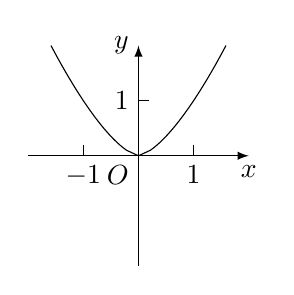
\begin{tikzpicture}[scale = 0.7, >=latex]
\draw [->] (-2,0) -- (2,0) node [below] {$x$};
\draw [->] (0,-2) -- (0,2) node [left] {$y$};
\draw (0,0) node [below left] {$O$};
\draw (1,0.2) -- (1,0) node [below] {$1$};
\draw (0.2,1) -- (0,1) node [left] {$1$};
\draw (-1,0.2) -- (-1,0) node [below] {$-1$};
\draw [domain = 0:4,samples = 400] plot ({\x^(1/3)},{\x^(1/2)});
\draw [domain = 0:4,samples = 400] plot ({-\x^(1/3)},{\x^(1/2)});
\end{tikzpicture}}{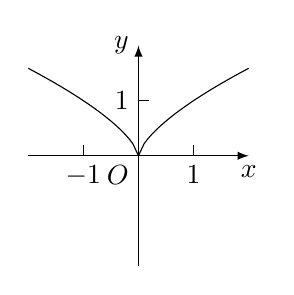
\begin{tikzpicture}[scale = 0.7, >=latex]
\draw [->] (-2,0) -- (2,0) node [below] {$x$};
\draw [->] (0,-2) -- (0,2) node [left] {$y$};
\draw (0,0) node [below left] {$O$};
\draw (1,0.2) -- (1,0) node [below] {$1$};
\draw (0.2,1) -- (0,1) node [left] {$1$};
\draw (-1,0.2) -- (-1,0) node [below] {$-1$};
\draw [domain = 0:4,samples = 400] plot ({\x^(1/2)},{\x^(1/3)});
\draw [domain = 0:4,samples = 400] plot ({-\x^(1/2)},{\x^(1/3)});
\end{tikzpicture}}{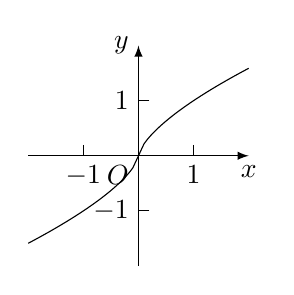
\begin{tikzpicture}[scale = 0.7, >=latex]
\draw [->] (-2,0) -- (2,0) node [below] {$x$};
\draw [->] (0,-2) -- (0,2) node [left] {$y$};
\draw (0,0) node [below left] {$O$};
\draw (1,0.2) -- (1,0) node [below] {$1$};
\draw (0.2,1) -- (0,1) node [left] {$1$};
\draw (-1,0.2) -- (-1,0) node [below] {$-1$};
\draw (0.2,-1) -- (0,-1) node [left] {$-1$};
\draw [domain = 0:4,samples = 400] plot ({\x^(1/2)},{\x^(1/3)});
\draw [domain = 0:4,samples = 400] plot ({-\x^(1/2)},{-\x^(1/3)});
\end{tikzpicture}}
\item 幂函数$y=x^m$和$y=x^n$在第一象限内的图像$C_1$和$C_2$图像所示, 则$m,n$之间的关系是\bracket{20}.
\begin{center}
    \begin{tikzpicture}[>=latex]
        \draw [->] (-1,0) -- (3,0) node [below] {$x$};
        \draw [->] (0,-1) -- (0,3) node [left] {$y$};
        \draw (0,0) node [below left] {$O$};
        \draw (1,0.2) -- (1,0) node [below] {$1$};
        \draw (0.2,1) -- (0,1) node [left] {$1$};
        \draw [domain = 0.5:2, samples = 400] plot (\x,{\x^(-5/4)});
        \draw [domain = 0.5:2, samples = 400] plot ({\x^(-5/4)},\x);
        \draw (0.5,{0.5^(-5/4)}) node [right] {$C_2$} ({0.5^(-5/4)},0.5) node [above] {$C_1$};
    \end{tikzpicture}
\end{center}
\fourch{$n<m<0$}{$m<n<0$}{$n>m>0$}{$m>n>0$}
\item 图中, $C_1,C_2,C_3$为幂函数$y=x^a$在第一象限的图像, 则解析式中的指数$\alpha$依次可以取\bracket{20}.
\begin{center}
    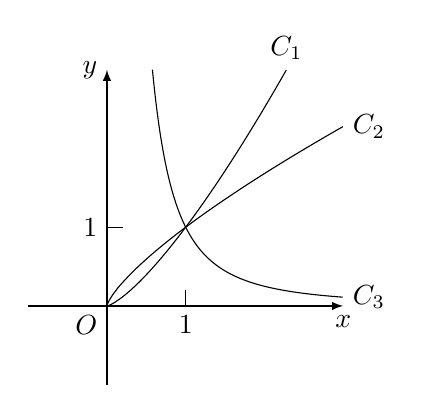
\begin{tikzpicture}[>=latex]
        \draw [->] (-1,0) -- (3,0) node [below] {$x$};
        \draw [->] (0,-1) -- (0,3) node [left] {$y$};
        \draw (0,0) node [below left] {$O$};
        \draw (1,0.2) -- (1,0) node [below] {$1$};
        \draw (0.2,1) -- (0,1) node [left] {$1$};
        \draw [domain = {sqrt(3)/3}:3, samples = 400] plot (\x,{\x^(-2)});
        \draw [domain = 0:3, samples = 400] plot (\x,{\x^(3/4)});
        \draw [domain = 0:{3^(3/4)}, samples = 400] plot (\x,{\x^(4/3)});
        \draw (3,{1/9}) node [right] {$C_3$} (3,{3^(3/4)}) node [right] {$C_2$} ({3^(3/4)},3) node [above] {$C_1$};
    \end{tikzpicture}
\end{center}
\fourch{$\dfrac 43,-2,\dfrac 34$}{$-2,\dfrac 34,\dfrac 43$}{$-2,\dfrac 43,\dfrac 34$}{$\dfrac 34,\dfrac 43,-2$}
\item 函数$y=x^{\frac 56}$的定义域为\blank{50}, 值域为\blank{50}.
\item 函数$y=x^{\frac 35}$的定义域为\blank{50}, 值域为\blank{50}.
\item 函数$y=x^{\frac 85}$的定义域为\blank{50}, 值域为\blank{50}.
\item 函数$y=x^{-\frac 54}$的定义域为\blank{50}, 值域为\blank{50}.
\item 函数$y=x^{-\frac 53}$的定义域为\blank{50}, 值域为\blank{50}.
\item 函数$y=x^{-\frac 23}$的定义域为\blank{50}, 值域为\blank{50}.
\item 函数$y=-2(x+5)^{-\frac 14}$的定义域为\blank{50}, 值域为\blank{50}.
\item 函数$y=5(2x-1)^{\frac 34}$的定义域为\blank{50}, 值域为\blank{50}.
\item 将下列函数图像的标号, 填在相应函数后面的横线上:\\
(1) $y=x^{\frac 23}$:\blank{50}; (2) $y=x^{-2}$:\blank{50}; (3) $y=x^{\frac 12}$:\blank{50};\\
(4) $y=x^{-1}$:\blank{50}; (5) $y=x^{\frac 13}$:\blank{50}; (6)$y=x^{\frac 32}$:\blank{50};\\ (7)$y=x^{\frac 43}$:\blank{50}; (8)$y=x^{-\frac 12}$:\blank{50}; (9)$y=x^{\frac 53}$:\blank{50}.
\begin{center}
    \begin{tikzpicture}[>=latex,scale = 0.6]
        \draw [->] (-2.5,0) -- (2.5,0) node [below] {$x$};
        \draw [->] (0,-2.5) -- (0,2.5) node [left] {$y$};
        \draw (0,0) node [below left] {$O$};
        \draw (0.2,1) -- (0,1) node [left] {$1$} (0.2,-1) -- (0,-1) node [left] {$-1$};
        \draw (1,0.2) -- (1,0) node [below] {$1$} (-1,0.2) -- (-1,0) node [below] {$1$};
        \draw (0,-2.5) node [below] {(A)};
        \draw [domain = 0:2.4, samples = 400] plot (\x,{\x^(1/2)});
    \end{tikzpicture}
    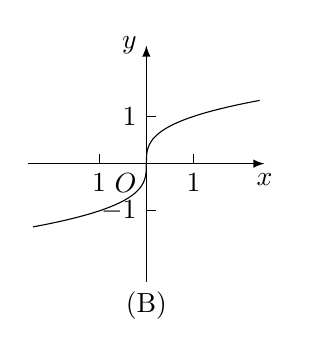
\begin{tikzpicture}[>=latex,scale = 0.6]
        \draw [->] (-2.5,0) -- (2.5,0) node [below] {$x$};
        \draw [->] (0,-2.5) -- (0,2.5) node [left] {$y$};
        \draw (0,0) node [below left] {$O$};
        \draw (0,-2.5) node [below] {(B)};
        \draw (0.2,1) -- (0,1) node [left] {$1$} (0.2,-1) -- (0,-1) node [left] {$-1$};
        \draw (1,0.2) -- (1,0) node [below] {$1$} (-1,0.2) -- (-1,0) node [below] {$1$};
        \draw [domain = 0:2.4, samples = 400] plot (\x,{\x^(1/3)});
        \draw [domain = 0:2.4, samples = 400] plot (-\x,{-\x^(1/3)});
    \end{tikzpicture}
    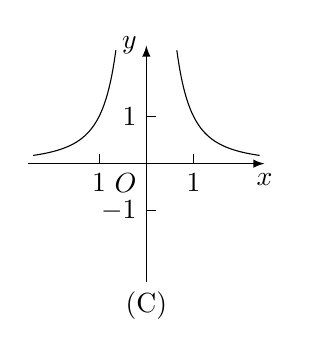
\begin{tikzpicture}[>=latex,scale = 0.6]
        \draw [->] (-2.5,0) -- (2.5,0) node [below] {$x$};
        \draw [->] (0,-2.5) -- (0,2.5) node [left] {$y$};
        \draw (0,0) node [below left] {$O$};
        \draw (0,-2.5) node [below] {(C)};
        \draw (0.2,1) -- (0,1) node [left] {$1$} (0.2,-1) -- (0,-1) node [left] {$-1$};
        \draw (1,0.2) -- (1,0) node [below] {$1$} (-1,0.2) -- (-1,0) node [below] {$1$};
        \draw [domain = {1/sqrt(2.4)}:2.4, samples = 400] plot (\x,{\x^(-2)});
        \draw [domain = {1/sqrt(2.4)}:2.4, samples = 400] plot (-\x,{\x^(-2)});
    \end{tikzpicture}\\
    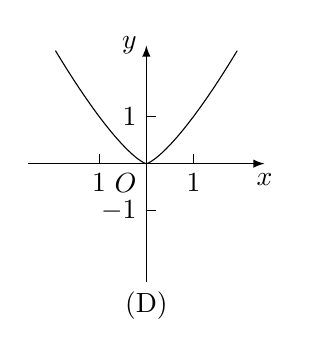
\begin{tikzpicture}[>=latex,scale = 0.6]
        \draw [->] (-2.5,0) -- (2.5,0) node [below] {$x$};
        \draw [->] (0,-2.5) -- (0,2.5) node [left] {$y$};
        \draw (0,0) node [below left] {$O$};
        \draw (0,-2.5) node [below] {(D)};
        \draw (0.2,1) -- (0,1) node [left] {$1$} (0.2,-1) -- (0,-1) node [left] {$-1$};
        \draw (1,0.2) -- (1,0) node [below] {$1$} (-1,0.2) -- (-1,0) node [below] {$1$};
        \draw [domain = 0:{2.4^(3/4)}, samples = 400] plot (\x,{\x^(4/3)});
        \draw [domain = 0:{2.4^(3/4)}, samples = 400] plot (-\x,{\x^(4/3)});
    \end{tikzpicture}
    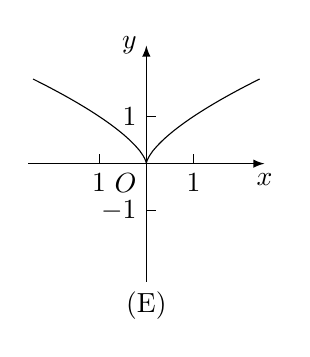
\begin{tikzpicture}[>=latex,scale = 0.6]
        \draw [->] (-2.5,0) -- (2.5,0) node [below] {$x$};
        \draw [->] (0,-2.5) -- (0,2.5) node [left] {$y$};
        \draw (0,0) node [below left] {$O$};
        \draw (0,-2.5) node [below] {(E)};
        \draw (0.2,1) -- (0,1) node [left] {$1$} (0.2,-1) -- (0,-1) node [left] {$-1$};
        \draw (1,0.2) -- (1,0) node [below] {$1$} (-1,0.2) -- (-1,0) node [below] {$1$};
        \draw [domain = 0:2.4, samples = 400] plot (\x,{\x^(2/3)});
        \draw [domain = 0:2.4, samples = 400] plot (-\x,{\x^(2/3)});
    \end{tikzpicture}
    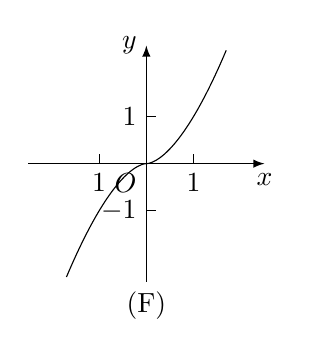
\begin{tikzpicture}[>=latex,scale = 0.6]
        \draw [->] (-2.5,0) -- (2.5,0) node [below] {$x$};
        \draw [->] (0,-2.5) -- (0,2.5) node [left] {$y$};
        \draw (0,0) node [below left] {$O$};
        \draw (0,-2.5) node [below] {(F)};
        \draw (0.2,1) -- (0,1) node [left] {$1$} (0.2,-1) -- (0,-1) node [left] {$-1$};
        \draw (1,0.2) -- (1,0) node [below] {$1$} (-1,0.2) -- (-1,0) node [below] {$1$};
        \draw [domain = 0:{2.4^(3/5)}, samples = 400] plot (\x,{\x^(5/3)});
        \draw [domain = 0:{2.4^(3/5)}, samples = 400] plot (-\x,{-\x^(5/3)});
    \end{tikzpicture}\\
    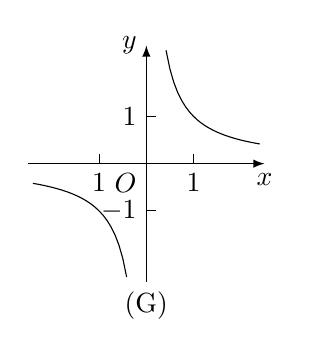
\begin{tikzpicture}[>=latex,scale = 0.6]
        \draw [->] (-2.5,0) -- (2.5,0) node [below] {$x$};
        \draw [->] (0,-2.5) -- (0,2.5) node [left] {$y$};
        \draw (0,0) node [below left] {$O$};
        \draw (0,-2.5) node [below] {(G)};
        \draw (0.2,1) -- (0,1) node [left] {$1$} (0.2,-1) -- (0,-1) node [left] {$-1$};
        \draw (1,0.2) -- (1,0) node [below] {$1$} (-1,0.2) -- (-1,0) node [below] {$1$};
        \draw [domain = {1/2.4}:2.4] plot (\x,{1/\x});
        \draw [domain = {1/2.4}:2.4] plot (-\x,{-1/\x});
    \end{tikzpicture}
    \begin{tikzpicture}[>=latex,scale = 0.6]
        \draw [->] (-2.5,0) -- (2.5,0) node [below] {$x$};
        \draw [->] (0,-2.5) -- (0,2.5) node [left] {$y$};
        \draw (0,0) node [below left] {$O$};
        \draw (0,-2.5) node [below] {(H)};
        \draw (0.2,1) -- (0,1) node [left] {$1$} (0.2,-1) -- (0,-1) node [left] {$-1$};
        \draw (1,0.2) -- (1,0) node [below] {$1$} (-1,0.2) -- (-1,0) node [below] {$1$};
        \draw [domain = {1/2.4^2}:2.4] plot (\x,{1/\x^(1/2)});
    \end{tikzpicture}
    \begin{tikzpicture}[>=latex,scale = 0.6]
        \draw [->] (-2.5,0) -- (2.5,0) node [below] {$x$};
        \draw [->] (0,-2.5) -- (0,2.5) node [left] {$y$};
        \draw (0,0) node [below left] {$O$};
        \draw (0,-2.5) node [below] {(I)};
        \draw (0.2,1) -- (0,1) node [left] {$1$} (0.2,-1) -- (0,-1) node [left] {$-1$};
        \draw (1,0.2) -- (1,0) node [below] {$1$} (-1,0.2) -- (-1,0) node [below] {$1$};
        \draw [domain = 0:{2.4^(2/3)}] plot (\x,{\x^(3/2)});
    \end{tikzpicture}
\end{center}
\item 若幂函数$y=x^n$的图像在$0<x<1$时位于直线$y=x$的下方, 则$n$的取值范围是\blank{50}.
\item 若幂函数$y=x^n$的图像在$0<x<1$时位于直线$y=x$的上方, 则$n$的取值范围是\blank{50}.
\item 函数$f(x)=x^{k^2-2k-3}$($k\in \mathbf{Z}$)的图像如图所示, 则$k=$\blank{50}.
\begin{center}
    \begin{tikzpicture}[>=latex]
        \draw [->] (-2.5,0) -- (2.5,0) node [below] {$x$};
        \draw [->] (0,-0.5) -- (0,2.5) node [left] {$y$};
        \draw (0,0) node [below left] {$O$};
        \draw (0,-0.5) node [below] {(C)};
        \draw (0.2,1) -- (0,1) node [left] {$1$};
        \draw (1,0.2) -- (1,0) node [below] {$1$} (-1,0.2) -- (-1,0) node [below] {$1$};
        \draw [domain = {1/2.4^(1/4)}:2.4, samples = 400] plot (\x,{\x^(-4)});
        \draw [domain = {1/2.4^(1/4)}:2.4, samples = 400] plot (-\x,{\x^(-4)});
    \end{tikzpicture}
\end{center}
\item 幂函数$y=x^p$与$y=x^q$的图像都通过定点\blank{50}, 它们在第一象限部分关于直线$y=x$对称, 则$p,q$应满足的条件是\blank{50}.
\item 若实数$a$满足$2.4^a>2.5^a$, 求$a$的取值范围.
\item 若实数$a$满足$(\dfrac 34)^{-a}>(\dfrac 43)^{-a}$, 求$a$的取值范围.
\item 若实数$a$满足$a^{-2}>3^{-2}$, 求$a$的取值范围.
\item 若实数$a$满足$0.01^{-3}>a^{-3}$, 求$a$的取值范围.
\item 将$2.5^{\frac 23}$, $(-1.4)^{\frac 23}$, $(-3)^{\frac 13}$从小到大排列:\blank{50}.
\item 将$4.1^{\frac 25}$, $3.8^{-\frac 23}$, $(-1.9)^{\frac 35}$从小到大排列:\blank{50}.
\item 将$0.16^{-\frac 34}$, $0.5^{-\frac 32}$, $6.25^{\frac 38}$从小到大排列:\blank{50}.
\item 已知函数$y=x^{n^2-2n-3}$($n\in \mathbf{Z}$)的图像与两坐标轴都无公共点, 且其图像关于$y$轴对称, 求$n$的值, 并画出相应的函数图像.
\item 函数$y=\sqrt {x^2+2x-3}$为减函数的区间是\bracket{20}.
\fourch{$(-\infty ,-3]$}{$[-1,+\infty)$}{$(-\infty ,-1]$}{$[1,+\infty)$}
\item 若函数$y=(2k+1)x+b$在$(-\infty,+\infty)$上是减函数, 则\bracket{20}.
\fourch{$k>\dfrac 12$}{$k<\dfrac 12$}{$k>-\dfrac 12$}{$k<-\dfrac 12$}
\item 若函数$f(x)=4x^2-mx+5$在区间$[-2,+\infty)$上是增函数, 在区间$(-\infty ,-2]$上是减函数, 则$f(1)$等于\bracket{20}.
\fourch{$-7$}{$1$}{$17$}{$25$}
\item 若函数$y=x^2+2(a-2)x+5$在区间$(4,+\infty)$上是增函数, 则实数$a$的取值范围是\bracket{20}.
\fourch{$a\le -2$}{$a\ge -2$}{$a\le -6$}{$a\ge -6$}
\item 下列函数中, 在区间$(0,2)$上为增函数的是\bracket{20}.
\fourch{$y=-3x+1$}{$y=\sqrt[3]x$}{$y=x^2-4x+3$}{$y=\dfrac 4x$}
\item 若函数$f(x)$在定义域$\mathbf{R}$上为增函数, 且$f(x)<0$, 则下列函数在$\mathbf{R}$上为增函数的是\bracket{20}.
\fourch{$y=|f(x)|$}{$y=\dfrac 1{f(x)}$}{$y=[ f(x) ]^2$}{$y=[ f(x) ]^3$}
\item 函数$y=\dfrac 1{\sqrt {x^2-4x+5}}$为增函数的区间是\blank{50}, 为减函数的区间是\blank{50}.
\item 函数$y=\dfrac 1{\sqrt {3+2x-x^2}}$为增函数的区间是\blank{50}.
\item 函数$y=|3x-5|$为减函数的区间是\blank{50}.
\item 函数$y=|x^2-2x-3|$为增函数的区间是\blank{50}.
\item 函数$y=\dfrac{1-x}{1+x}$为减函数的区间是\blank{50}.
\item 定义在$[1, 3]$上的函数$f(x)$为减函数, 求满足不等式$f(1-a)-f(3-a^2)>0$的解集.
\item 已知$f(x)=-x^3-x+1$($x\in \mathbf{R}$), 求证$y=f(x)$在定义域上为减函数.
\item 求证: 函数$f(x)=x+\dfrac 1x$在$(0, 1)$上是减函数, 在$(1,+\infty)$上是增函数.
\item 求证: $f(x)=\sqrt x-\dfrac 1x$在定义域上是增函数.
\item 已知常数$m,n$满足$mn<2$, 求证: 函数$f(x)=\dfrac{mx+1}{2x+n}$在$(-\dfrac n2,+\infty)$上为减函数.
\item 已知$f(x)=x^2+1$, $g(x)=x^4+2x^2+2$, 是否存在实数$\lambda$, 使得$F(x)=g(x)-\lambda f(x)$在$(-\infty ,-1)$上是减函数, 在$(-1,0)$上是增函数? 说明理由.
\item 已知函数$f(x)$在区间$(-\infty ,+\infty)$上是增函数, 又实数$a,b$满足$a+b\ge 0$, 求证: $f(a)+f(b)\ge f(-a)+f(-b)$.
\item $f(x)$是定义在$\mathbf{R}^+$的增函数, 且$f(\dfrac xy)=f(x)-f(y)$.\\
(1) 求$f(1)$的值;\\
(2) 若$f(6)=1$, 解不等式$f(x+3)-f(\dfrac 1x)<2$.
\item 若$f(x)=(m-1)x^2+3mx+3$为偶函数, 则$f(x)$在区间$(-4,2)$上\bracket{20}.
\twoch{是增函数}{是减函数}{先是增函数后是减函数}{先是减函数后是增函数}
\item 函数$f(x)=\begin{cases}   1-x, & x>0,  \\ 0, & x=0,  \\1+x, & x<0,  \end{cases}$则该函数\bracket{20}.
\twoch{是奇函数, 但不是偶函数}{是偶函数, 但不是奇函数}{既是奇函数, 也是偶函数}{既不是奇函数, 也不是偶函数}
\item 下列函数中既是奇函数, 又在定义域上为增函数的是\bracket{20}.
\fourch{$f(x)=3x+1$}{$f(x)=\dfrac 1x$}{$f(x)=1-\dfrac 1x$}{$f(x)=x^3$}
\item 若$f(x)$为定义在区间$[-6, 6]$上的偶函数, 且满足$f(3)>f(1)$, 则恒成立的是\bracket{20}.
\fourch{$f(-1)<f(3)$}{$f(0)<f(6)$}{$f(3)>f(2)$}{$f(2)>f(0)$}
\item 函数$f(x)=\dfrac{\sqrt {1-x^2}}{2-|x+2|}$\bracket{20}.
\twoch{是奇函数, 但不是偶函数}{是偶函数, 但不是奇函数}{既是奇函数, 又是偶函数}{既不是奇函数, 也不是偶函数}
\item 已知$f(x)$是奇函数, 则下列各点中在函数$y=f(x)$的图像上的点的是\bracket{20}.
\fourch{$(a,f(-a))$}{$(-a,-f(a))$}{$(\dfrac 1a,-f(\dfrac 1a))$}{$(-\sin a,-f(-\sin a))$}
\item 若$f(x)$是定义在$\mathbf{R}$上的偶函数, 且当$x<0$时, $f(x)=2x-3$, 则当$x>0$时, $f(x)=$\blank{50}.
\item 若奇函数$f(x)$的定义域是$\mathbf{R}$, 则$f(0)=$\blank{50}.
\item 若奇函数$f(x)$在区间$[-3, -1]$上是增函数, 且有最大值$-2$, 则$f(x)$在$[1, 3]$上是\blank{50}函数(填``增''或``减''), 且最小值等于\blank{50}.
\item 设$f(x)$为定义在$\mathbf{R}$上的偶函数, 且$f(x)$在$[0,+\infty)$上是增函数, 则$f(-4)$, $f(-2)$, $f(3)$由小到大的排列顺序为\blank{50}.
\item 若函数$f(x)=x^5+px^3+qx-8$满足$f(-2)=10$, 则$f(2)=$\bracket{20}.
\fourch{$10$}{$-10$}{$-26$}{$-18$}
\item 设$f(x)$在$R$上是奇函数, 且当$x\in [0,+\infty)$时, $f(x)=x(1+\sqrt[3]x)$, 那么当$x\in (-\infty ,0)$时, $f(x)=$\bracket{20}.
\fourch{$-x(1+\sqrt[3]x)$}{$x(1+\sqrt[3]x)$}{$-x(1-\sqrt[3]x)$}{$x(1-\sqrt[3]x)$}
\item 若函数$f(x)=8+2x-x^2$, 记$g(x)=f(2-x^2)$, 则$g(x)$\bracket{20}.
\fourch{在(-2, 0)上是增函数}{在(0, 2)上是增函数}{在(-1, 0)上是减函数}{在(0, 1)上是减函数}
\item 函数$f(x)=x|x|-2x$是\bracket{20}.
\twoch{偶函数, 且在(-1, 1)上是增函数}{奇函数, 且在(-1, 1)上是减函数}{偶函数, 且在(-1, 1)上是减函数}{奇函数, 且在(-1, 1)上是增函数}
\item 若函数$y=f(x)$是偶函数, 其图像与$x$轴有四个交点, 则方程$f(x)=0$的所有实数根之和为\bracket{20}.
\fourch{$4$}{$2$}{$1$}{$0$}
\item 函数$f(x)=\dfrac x{2^{1+x}+2^{1-x}}$\bracket{20}.
\twoch{是奇函数, 但不是偶函数}{是偶函数, 但不是奇函数}{既是奇函数, 又是偶函数}{既不是奇函数, 也不是偶函数}
\item 已知奇函数$f(x)$在$x>0$时的表达式为$f(x)=2x-\dfrac 12$, 则当$x\le -\dfrac 14$时, 恒有\bracket{20}.
\fourch{$f(x)>0$}{$f(x)<0$}{$f(x)-f(-x)\le 0$}{$f(x)-f(-x)>0$}
\item $f(x)+f(2-x)+2=0$对任何实数$x$都成立, 则$f(x)$的图像\bracket{20}.
\twoch{关于直线$x=1$成轴对称图形}{关于直线$x=2$成轴对称图形}{关于点$(1, -1)$成中心对称图形}{关于点$(-1,1)$成中心对称图形}
\item 已知$f(x),g(x)$都是定义在$\mathbf{R}$上的函数, $f(x)$为奇函数, $g(x)$为偶函数, 且$f(x)\cdot g(x)$恒不为$0$, 判断下列函数的奇偶性:
(1)$f(x)+g(x)$:\blank{50}; (2)$f(x)\cdot g(x)$:\blank{50}; (3)$f[f(x)]$:\blank{50}; (4)$f[g(x)]$:\blank{50}; (5)$g[f(x)]$:\blank{50}; (6)$g[g(x)]$:\blank{50}.
\item 判断函数$f(x)=5$的奇偶性:\blank{50}.
\item 判断函数$f(x)=\sqrt {x^2-1}+\sqrt {1-x^2}$的奇偶性:\blank{50}.
\item 判断函数$f(x)=x^2-2x^2+3$的奇偶性:\blank{50}.
\item 判断函数$x\in [-4,4)$的奇偶性:\blank{50}.
\item 判断函数$f(x)=|3x+2|-|3x-2|$的奇偶性:\blank{50}.
\item 判断函数$f(x)=\dfrac{x^2(x-1)}{x-1}$的奇偶性:\blank{50}.
\item 判断函数$f(x)=\dfrac 12[g(x)-g(-x)]$的奇偶性:\blank{50}.
\item 求证: 函数$f(x)=\dfrac{x+1+\sqrt {1+x^2}}{x-1+\sqrt {1+x^2}}$是奇函数.
\item 求证: 函数$f(x)=\begin{cases}
   x(1-x), &  x>0,  \\ x(1+x), &  x<0  \end{cases}$是奇函数.
\item 已知奇函数$f(x)$在定义域$(-l, l)$上是减函数, 求满足$f(1-m)+f(1-m^2)<0$的实数$m$的取值范围.
\item 已知偶函数$f(x)$在$[0,+\infty)$上是增函数.求不等式$f(2x+5)<f(x^2+2)$的解集.
\item 是否存在既是奇函数又是偶函数的函数? 说明理由
\item 求证: 定义域为$(-l,l)$的任何函数都能表示成一个奇函数与一个偶函数之和.
\item 下列函数中有反函数的是\bracket{20}.
\fourch{$y=3+\sqrt {x^2+5}$}{$y=\dfrac 1{x^2+1}$}{$y=\sqrt [3]{2x-1}+2$}{$y=\begin{cases}
   x^2-3, &  x\ge 0,  \\3x, &  x<0  \end{cases}$}
\item 函数$y=\sqrt {x^2-2x+3}$($x\le 1$)的反函数的定义域是\bracket{20}.
\fourch{$[0,+\infty)$}{$(2,+\infty)$}{$(-\infty ,1]$}{$[\sqrt 2,+\infty)$}
\item 设$f(x)=\dfrac{2x+1}{4x+3}$($x\in \mathbf{R}$, 且$x\ne -\dfrac 34$), 则$f^{-1}(2)$的值等于\bracket{20}.
\fourch{$-\dfrac 56$}{$-\dfrac 25$}{$\dfrac 25$}{$\dfrac 5{11}$}
\item 函数$y=x^2+2x$($x<-1$)的反函数是\bracket{20}.
\twoch{$y=\sqrt {x+1}-1$($x<-1$)}{$y=\sqrt {x+1}-1$($x>-1$)}{$y=-\sqrt {x+1}-1$($x<-1$)}{$y=-\sqrt {x+1}-1$($x>-1$)}
\item 若函数$y=g(x)$的图像与函数$f(x)=(x-1)^2$($x\le 1$)的图像关于直线$y=x$对称.则$g(x)$的表达式是\bracket{20}.
\twoch{$g(x)=1-\sqrt x$($x\ge 0$)}{$g(x)=1+\sqrt x$($x\ge 0$)}{$g(x)=\sqrt {1-x}$($x\le 1$)}{$g(x)=\sqrt {1+x}$($x\ge -1$)}
\item 函数$y=\dfrac{ax+b}{cx+1}$($a\ne bc$)的反函数是$y=\dfrac{x+2}{3x+1}$, 则的$a,b,c$值依次为\bracket{20}.
\fourch{$1,-2,-3$}{$-1,2,3$}{$-1, 2, -3$}{$1, 2, 3$}
\item 若函数$f(x)=\dfrac{x-2}{x+m}$的反函数$f^{-1}(x)=f(x)$, 则$m$的值是\bracket{20}.
\fourch{$1$}{$-1$}{$2$}{$-2$}
\item 若函数$f(x)$的图像经过点$(0, -1)$, 则函数$f(x+4)$的反函数的图像必经过点\bracket{20}.
\fourch{$(—1,4)$}{$(-4,-1)$}{$(-1,-4)$}{$(1,-4)$}
\item 已知函数$y=-\sqrt {1-x^2}$的反函数是$y=-\sqrt {1-x^2}$, 则原函数的定义域``最大''可以是\blank{50}.
\item 已知函数$y=\dfrac 13x+m$与$y=nx-6$互为反函数, 则$m=$\blank{50}, $n=$\blank{50}.
\item 若点$(1, 2)$既在函数$y=\sqrt {ax+b}$的图像上.又在其反函数的图像上, 则$a=$\blank{50}, $b=$\blank{50}.
\item 若$y=\dfrac{1+x}{1-x}$($x\ne 1$), 则其反函数$f^{-1}(x)=$\blank{50}.
\item 若$f(x)=x^{\frac 23}$($x\le 0$), 则其反函数$f^{-1}(x)=$\blank{50}.
\item 若$f(x)=-\sqrt {1-x^2}$($0\le x\le 1$), 则其反函数$f^{-1}(x)=$\blank{50}.
\item 若$f(x)=\sqrt {x^2-4}$($x\le -2$), 则其反函数$f^{-1}(x)=$\blank{50}.
\item 若$f(x)=\begin{cases}
   x^2, & x\le 0,  \\ -3x, & x>0,  \end{cases}$ 则其反函数$f^{-1}(x)=$\blank{50}.
\item 若$f(x)=\begin{cases}
   x, & 0\le x\le 1,  \\1-x, & -1\le x<0,  \end{cases}$ 则其反函数$f^{-1}(x)=$\blank{50}.
\item 若$f(x)=\begin{cases}
   x^2-1,  & x\ge 0,  \\2x-1, & x<0,  \end{cases}$ 则其反函数$f^{-1}(x)=$\blank{50}.
\item 已知函数$f(x)=\dfrac{x+1}{x-1}$, $g(x)=f^{-1}(-x)$, 则$g(x)$\bracket{20}.
\twoch{在$(-\infty ,+\infty)$上是增函数}{在$(-\infty ,-1)$上是增函数}{在$(1,+\infty)$上是减函数}{在$(-\infty ,-1)$上是减函数}
\item 若函数$y=\sqrt {x-m}$与其反函数的图像有公共点, 则$m$的取值范围是\bracket{20}.
\fourch{$m\ge \dfrac 14$}{$m\le \dfrac 14$}{$m\ge 0$}{$m\le 0$}
\item 已知$y=g(x)$是函数$y=f(x)$的反函数, 又$y=h(x)$与$y=g(x)$的图像关于原点$O(0,0)$对称, 则$h(x)$的表达式是\bracket{20}.
\fourch{$y=f^{-1}(x)$}{$y=-f^{-1}(x)$}{$y=f^{-1}(-x)$}{$y=-f^{-1}(-x)$}
\item 若幂函数$f(x)$是奇函数, 则$f^{-1}(1)=$\blank{50}, $f^{-1}(-1)=$\blank{50}.
\item 若$f(x)=\dfrac{2x-1}{x+a}$存在反函数, 则实数$a$的取值范围是\blank{50}.
\item 若$f(x)=2x^2-4x+9$($x\ge 1$), 且满足$f^{-1}(a+1)=3$, 则$f(a)=$\blank{50}.
\item 已知定义域为$(-\infty ,0]$的函数$f(x)$满足$f(x-1)=x^2-2x$, 则$f^{-1}(-\dfrac 12)=$\blank{50}.
\item 求函数$f(x)=\begin{cases}
   x+1, &  x>0,  \\ x-1, &  x<0  \end{cases}$的反函数, 并作出其反函数的图像.
\item 已知函数$f(x)=x^2+2x+1$.\\
(1) 若函数的定义域是$(-\infty ,+\infty)$, 这个函数有没有反函数?\\
(2) 若函数的定义域是$[0,+\infty)$, 求其反函数;\\
(3) 若函数的定义域是$(-\infty ,-1]$, 求其反函数.
\item 若关于$x$的方程$x^2+2(m+3)x+2m+14=0$有两个实数根, 且一个比$4$大, 另一个比$4$小, 求实数$m$的取值范围.
\item 若关于$x$的方程$x^2+2mx-(m-12)=0$的两根都大于$2$, 求实数$m$的取值范围.
\item 若关于$x$的方程$7x^2-(m+13)x+m^2-m-2=0$的两实数根$\alpha ,\beta$满足$0<\alpha <1<\beta <2$, 求实数$m$的取值范围.
\item 若关于$x$的方程$2x^2-3x+2m=0$的两根均在$[-1, 1]$之间, 求实数$m$的取值范围.
\item 若关于$x$的方程$x^2+2mx+2m^2-1=0$至少有一负根, 求实数$m$的取值范围.
\item 若在区间$[-2, 2]$内恰有一个$x$的值满足方程$2mx^2-x-1=0$, 求实数$m$的取值范围.
\item 若关于$x$的方程$x^2+x=m+1$在$0<x\le 1$内有解, 求实数$m$的取值范围.
\item 就实数$k$的取值讨论下列关于$x$的方程解的情况:\\
(1) $x^2+2|x|-k=0$;\\
(2) $|x^2-2x-3|=k$.
\item 将下列各数从小到大排列: $(\dfrac 23)^{-\frac 13}$, $(\dfrac 35)^{\frac 12}$, $(\dfrac 25)^{\frac 12}$, $3^{\frac 13}$, $(\dfrac 32)^{\frac 23}$, $(-2)^3$, $(\dfrac 53)^{-\frac 13}$.\\
解答在这里  (1)与零比, 负数有$(-2)^3$.
(2)与$1$比, 小于$1$的数有$(\dfrac 35)^{\frac 12}$, $(\dfrac 25)^{\frac 12}$, $(\dfrac 53)^{-\frac 13}$.
利用幂函数$x^{\frac 12}$的性质, 得$(\dfrac 25)^{\frac 12}<(\dfrac 35)^{\frac 12}$, 再利用指数函数$(\dfrac 35)^x$的性质, 得$(\dfrac 35)^{\frac 12}<(\dfrac 35)^{\frac 13}=(\dfrac 53)^{-\frac 13}$, 所以$(\dfrac 25)^{\frac 12}<(\dfrac 35)^{\frac 12}<(\dfrac 53)^{-\frac 13}$;
(3)与$1$比, 大于$1$的数有$(\dfrac 23)^{-\frac 13}$, $3^{\frac 13}$, $(\dfrac 32)^{\frac 23}$.
利用指数函数$(\dfrac 32)^x$的性质, 得$(\dfrac 23)^{-\frac 13}=(\dfrac 32)^{\frac 13}<(\dfrac 32)^{\frac 23}$.
再利用幂函数$x^{\frac 23}$的性质, 得$(\dfrac 32)^{\frac 23}<(\sqrt 3)^{\frac 23}=3^{\frac 13}$, 所以$ (\dfrac 23)^{-\frac 13}<(\dfrac 32)^{\frac 23}<3^{\frac 13}$.
综上所述, 得$(-2)^3<(\dfrac 23)^{\frac 12}<(\dfrac 35)^{\frac 12}<(\dfrac 53)^{-\frac 13}<(\dfrac 23)^{-\frac 13}<(\dfrac 32)^{\frac 23}<3^{\frac 13}$.
\item 求函数$y=(\dfrac 12)^{-x^2+2x}$为增函数的区间.\\
解答在这里, 解法一  因为$ 0<\dfrac 12<1$,
所以$-x^2+2x$为减函数的区间为$[1,+\infty)$, 也就是$y$为增函数的区间.
解法二  因为$y=(\dfrac 12)^{-x^2+2x}=2^{x^2-2x}=2^{(x-1)^2-1}$,
所以$y$为增函数的区间就是$x^2-2x$为增函数的区间, 即$[1,+\infty)$.
\item 求函数$y=9^x-m\cdot 3^x+1$的最小值.\\
解答在这里  令$t=3^x$则函数为$y=t^2-mt+1=(t-\dfrac m2)^2+1-\dfrac{m^2}4$, 其图像的对称轴方程为$t=\dfrac m2$.
(1) 如下图左, 若$\dfrac m2>0$, 则当$t=\dfrac m2$时, $y_{\min }=1-\dfrac{m^2}4$.
\begin{center}
    \begin{tikzpicture}[>=latex]
        \draw [->] (-1,0) -- (3,0) node [below] {$t$};
        \draw [->] (0,-1) -- (0,3) node [left] {$y$};
        \draw (0,0) node [below left] {$O$};
        \draw [dashed, domain = -0.5:0, samples = 100] plot (\x,{(\x-1)^2/2+1});
        \draw [domain = 0:2.5, samples = 100] plot (\x,{(\x-1)^2/2+1});
        \draw [dashed] (1,-0.5) -- (1,2.5);
        \draw (1,0) node [below right] {$\frac{m}{2}$};
        \filldraw [white] (0,1.5) circle (0.05);
        \draw (0,1.5) circle (0.05);
    \end{tikzpicture}
    \begin{tikzpicture}[>=latex]
        \draw [->] (-3,0) -- (1,0) node [below] {$t$};
        \draw [->] (0,-1) -- (0,3) node [left] {$y$};
        \draw (0,0) node [below left] {$O$};
        \draw [dashed, domain = -2.5:0, samples = 100] plot (\x,{(\x+1)^2/2+1});
        \draw [domain = 0:0.5, samples = 100] plot (\x,{(\x+1)^2/2+1});
        \draw [dashed] (-1,-0.5) -- (-1,2.5);
        \draw (-1,0) node [below right] {$\frac{m}{2}$};
        \filldraw [white] (0,1.5) circle (0.05);
        \draw (0,1.5) circle (0.05);
    \end{tikzpicture}
\end{center}
(2) 如上图右, 若$\dfrac m2\le 0$, 则由于$t>0$, 函数无最小值.
\item 填写下表:
\begin{center}
    \begin{tabular}{|c|c|c|c|c|}
        \hline
        $x$	 & $f(x)=x^2$ & $f(x)-f(x-1)$ & $g(x)=2^x$ & $g(x)-g(x-1)$ \\ \hline
        $0$ & & & & \\ \hline
        $1$ & & & & \\ \hline
        $2$ & & & & \\ \hline
        $3$ & & & & \\ \hline
        $4$ & & & & \\ \hline
        $5$ & & & & \\ \hline
        $6$ & & & & \\ \hline
        $7$ & & & & \\ \hline
        $8$ & & & & \\ \hline
        $9$ & & & & \\ \hline
        $10$ & & & & \\ \hline
    \end{tabular}
\end{center}
(1) 比较$f(x)=x^2$与$g(x)=2^x$的函数值的大小;\\
(2) 比较$f(x)=x^2$与$g(x)=2^x$的函数值递增的快慢.
解答在这里,  经计算得下表:
\begin{center}
    \begin{tabular}{|c|c|c|c|c|}
        \hline
        $x$	 & $f(x)=x^2$ & $f(x)-f(x-1)$ & $g(x)=2^x$ & $g(x)-g(x-1)$ \\ \hline
        $0$ & $0$ &  & $1$ & \\ \hline 
        $1$ & $1$ & $1$ & $2$ & $1$ \\  \hline 
        $2$ & $2$ & $1$ & $4$ & $2$\\  \hline 
        $3$ & $9$ & $7$ & $8$ & $4$\\  \hline 
        $4$ & $16$ & $7$ & $16$ & $8$\\  \hline 
        $5$ & $25$ & $9$ & $32$ & $16$\\ \hline 
        $6$ & $36$ & $11$ & $64$ & $32$\\  \hline 
        $7$ & $49$ & $13$ & $128$ & $64$\\ \hline
        $8$ & $64$ & $15$ & $256$ & $128$\\  \hline 
        $9$ & $81$ & $17$ & $512$ & $256$\\  \hline 
        $10$ & $100$ & $19$ & $1024$ & $512$\\ \hline
    \end{tabular}
\end{center}
并描点得出函数$f(x)=x^2$与$g(x)=2^x$在同一个平面直角坐标系下的图像如图所示.
\begin{center}
    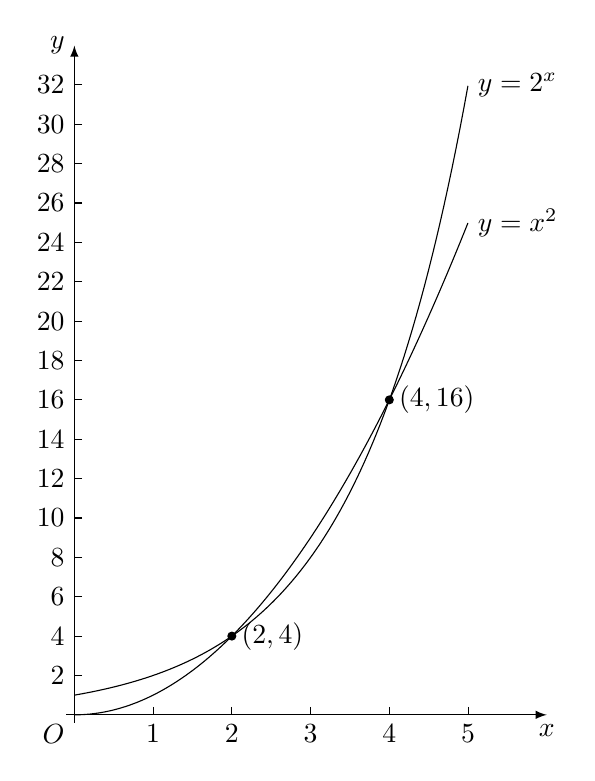
\begin{tikzpicture}[>=latex]
        \draw [->] (-0.1,0) -- (6,0) node [below] {$x$};
        \draw [->] (0,-0.1) -- (0,8.5) node [left] {$y$};
        \draw (0,0) node [below left] {$O$};
        \draw [domain = 0:5,samples = 100] plot (\x,{\x^2/4});
        \draw [domain = 0:5, samples = 100] plot (\x,{2^(\x)/4});
        \draw (5,{25/4}) node [right] {$y=x^2$} (5,8) node [right] {$y=2^x$};
        \filldraw (2,1) circle (0.05) node [right] {$(2,4)$} (4,4) circle (0.05) node [right] {$(4,16)$};
        \foreach \i in {1,2,...,5}{\draw (\i,0.1) -- (\i,0) node [below] {$\i$};};
        \foreach \i in {2,4,...,32}{\draw (0.1,\i/4) -- (0,\i/4) node [left] {$\i$};};
    \end{tikzpicture}
\end{center}
由表和图知:\\
(1) 当$0<x<2$时, $g(x)>f(x)$; 当$2<x<4$时, $f(x)>g(x)$; 当$x>4$时, $g(x)>f(x)$; 当$x=2$或$x=4$时, $f(x)=f(x)$.
(2) 当$x>4$时, $f(x)=x^2$的函数值递增的速度较$g(x)=2^x$慢.
\item 已知函数$f(x)=2x+1$, $g(x)=1.5^x$, $h(x)=x^{1.5}$, 试用数值计算比较三个函数在$[0,+\infty)$上的函数值的大小、图像递增的快慢. 并说明在函数图像上的表现.
解  列表并计算得:
\begin{center}
    \begin{longtable}{|c|c|c|c|c|c|c|}
        \hline
        $x$	 & $f(x)=2x+1$ & $f(x)-f(x-1)$ & $g(x)=1.5^x$ & $g(x)-g(x-1)$ & $h(x)=x^{1.5}$ & $h(x)-h(x-1)$ \\ \hline
        \endhead
        $0$ & $1$ & & $1$ & & $0$ &  \\ \hline
        $1$ & $3$ & $2$ & $1.5$ & $0.5$ & $1$ & $1$\\ \hline
        $2$ & $5$ & $2$ & $2.25$ & $0.75$ & $2.82842712$ & $1.82842712$\\ \hline
        $3$ & $7$ & $2$ & $3.375$ & $1.125$ & $5.19615242$ & $2.3677253$\\ \hline
        $4$ & $9$ & $2$ & $5.0625$ & $1.6875$ & $8$ & $2.80384758$\\ \hline
        $5$ & $11$ & $2$ & $7.59375$ & $2.53125$ & $11.1803399$ & $3.18033989$\\ \hline
        $6$ & $13$ & $2$ & $11.390625$ & $3.796875$ & $14.6969385$ & $3.51659857$\\ \hline
        $7$ & $15$ & $2$ & $17.085938$ & $5.6953125$ & $18.5202592$ & $3.82332072$\\ \hline
        $8$ & $17$ & $2$ & $25.628906$ & $8.5429688$ & $22.627417$ & $4.10715782$\\ \hline
        $9$ & $19$ & $2$ & $38.443359$ & $12.814453$ & $27$ & $4.372583$\\ \hline
        $10$ & $21$ & $2$ & $57.665039$ & $19.22168$ & $31.6227766$ & $4.6227766$\\ \hline
        $11$ & $23$ & $2$ & $86.497559$ & $28.83252$ & $36.4828727$ & $4.86009609$\\ \hline
        $12$ & $25$ & $2$ & $129.74634$ & $43.248779$ & $41.5692194$ & $5.08634669$\\ \hline
        $13$ & $27$ & $2$ & $194.61951$ & $64.873169$ & $46.8721666$ & $5.3029472$\\ \hline
        $14$ & $29$ & $2$ & $291.92926$ & $97.309753$ & $52.3832034$ & $5.51103683$\\ \hline
        $15$ & $31$ & $2$ & $437.89389$ & $145.96463$ & $58.0947502$ & $5.71154678$\\ \hline
        $16$ & $33$ & $2$ & $656.84084$ & $218.94695$ & $64$ & $5.90524981$\\ \hline
        $17$ & $35$ & $2$ & $985.26125$ & $328.42042$ & $70.0927956$ & $6.09279564$\\ \hline
        $18$ & $37$ & $2$ & $1477.8919$ & $492.63063$ & $76.3675324$ & $6.27473673$\\ \hline
        $19$ & $39$ & $2$ & $2216.8378$ & $738.94594$ & $82.8190799$ & $6.45154756$\\ \hline
        $20$ & $41$ & $2$ & $3325.2567$ & $1108.4189$ & $89.4427191$ & $6.62363917$\\ \hline
        $21$ & $43$ & $2$ & $4987.8851$ & $1662.6284$ & $96.2340896$ & $6.79137049$\\ \hline
        $22$ & $45$ & $2$ & $7481.8276$ & $2493.9425$ & $103.189147$ & $6.95505712$\\ \hline
        $23$ & $47$ & $2$ & $11222.741$ & $3740.9138$ & $110.304125$ & $7.11497832$\\ \hline
        $24$ & $49$ & $2$ & $16834.112$ & $5611.3707$ & $117.575508$ & $7.27138262$\\ \hline
        $25$ & $51$ & $2$ & $25251.168$ & $8417.0561$ & $125$ & $7.42449235$\\ \hline
        $26$ & $53$ & $2$ & $37876.752$ & $12625.584$ & $132.574507$ & $7.57450735$\\ \hline
        $27$ & $55$ & $2$ & $56815.129$ & $18938.376$ & $140.296115$ & $7.72160806$\\ \hline
        $28$ & $57$ & $2$ & $85222.693$ & $28407.564$ & $148.162073$ & $7.86595801$\\ \hline
        $29$ & $59$ & $2$ & $127834.04$ & $42611.346$ & $156.169779$ & $8.00770599$\\ \hline
        $30$ & $61$ & $2$ & $191751.06$ & $63917.02$ & $164.316767$ & $8.14698784$\\ \hline
        $\cdots$ & $\cdots$ & $\cdots$ & $\cdots$ & $\cdots$ & $\cdots$ & $\cdots$ \\ \hline
    \end{longtable}
\end{center}
得点$A,B,C,D$的横坐标分别约为$1.5,4.8, 6.5, 7.4$, 记作$x_A,x_B,x_C,x_D$.\\
(1) 三个函数的函数值的大小情况如下:\\
\textcircled{1} 当$0<x<x_A$时, $f(x)>g(x)>h(x)$;
\textcircled{2} 当$x_A<x<x_B$时, $f(x)>h(x)>g(x)$;
\textcircled{3} 由$x_B<x<x_C$时, $h(x)>f(x)>g(x)$;
\textcircled{4} 当$x_C<x<x_D$时, $h(x)>g(x)>f(x)$;
\textcircled{5} 当$x_D<x$时, $g(x)>h(x)>f(x)$;
\textcircled{6} 当$x=x_A$时, $f(x)>g(x)=h(x)$;
\textcircled{7} 当$x=x_B$时, $f(x)=h(x)>g(x)$;
\textcircled{8} 当$x=x_C$时, $f(x)=g(x)<h(x)$;
\textcircled{9} 当$x=x_D$时, $f(x)<g(x)=g(x)$.\\
(2) 它们在同一个平面直角坐标系下的图像如图14所示.
\begin{center}
    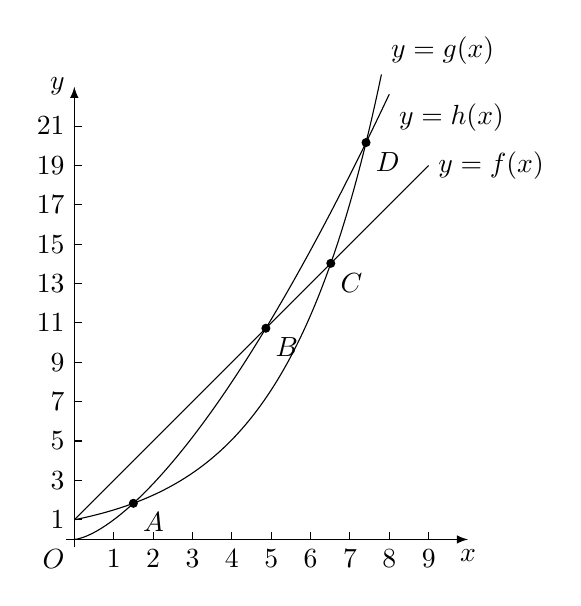
\begin{tikzpicture}[>=latex]
        \draw [->] (-0.1,0) -- (5,0) node [below] {$x$};
        \draw [->] (0,-0.1) -- (0,5.75) node [left] {$y$};
        \draw (0,0) node [below left] {$O$};
        \draw [domain = 0:9,samples = 100, name path = firstorder] plot ({\x/2},{(2*\x+1)/4});
        \draw (4.5,{19/4}) node [right] {$y=f(x)$};
        \draw [domain = 0:7.8, samples = 100, name path = exponential] plot ({\x/2},{1.5^(\x)/4}); 
        \draw (3.9,{1.5^7.8/4}) node [above right] {$y=g(x)$};
        \draw [domain = 0:8, samples = 100, name path = power] plot ({\x/2},{\x^(3/2)/4});
        \draw (4,{8^(3/2)/4}) node [below right] {$y=h(x)$};
        \path [name intersections = {of = firstorder and exponential, by = {T,C}}];
        \path [name intersections = {of = firstorder and power, by = B}];
        \path [name intersections = {of = exponential and power, by = {A,D}}];
        \filldraw (A) circle (0.05) node [below right] {$A$};
        \filldraw (B) circle (0.05) node [below right] {$B$};
        \filldraw (C) circle (0.05) node [below right] {$C$};
        \filldraw (D) circle (0.05) node [below right] {$D$};
        \foreach \i in {1,2,...,9}{\draw (\i/2,0.1) -- (\i/2,0) node [below] {$\i$};};
        \foreach \i in {1,3,...,21}{\draw (0.1,\i/4) -- (0,\i/4) node [left] {$\i$};};
    \end{tikzpicture}
\end{center}
由表格及图像可看出, 三个函数的函数值变化及相应增量规律为: 随着$x$的增大, 直线型均匀上升, 增量恒定; 指数型急剧上升, 在区间$[0,+\infty)$上递增增量快速增大; 幂函数型虽上升较快, 但随着$x$的不断增大上升趋势远不如指数型, 几乎微不足道, 其增量缓慢递增. 
\item 已知函数$f(x)=4+a^{x-1}$的图像恒过记点$P$, 则点$P$的坐标是\bracket{20}.
\fourch{$(1, 5)$}{$(1, 4)$}{$(0, 4)$}{$(4, 0)$}
\item 下列函数中, 值域为$(0,+\infty)$的函数是\bracket{20}.
\fourch{$y=(\dfrac 18)^{2-x}$}{$y=\sqrt {1-3^x}$}{$y=\sqrt {(\dfrac 13)^x-1}$}{$y=2^{\frac 1{3-x}}$}
\item 若$0<a<1$, 记$m=a^{-1}$, $n=a^{-\frac 43}$, $p=a^{-\frac 13}$, 则$m,n,p$的大小关系是\bracket{20}.
\fourch{$m<n<p$}{$m<p<n$}{$n<m<p$}{$p<m<n$}
\item 下列函数式中, 满足$f(x+1)=2f(x)$的$f(x)$是\bracket{20}.
\fourch{$\dfrac 12(x+1)$}{$x+\dfrac 14$}{$2^x$}{$2^{-x}$}
\item 若$f(x)=\dfrac{\mathrm{e}^x-\mathrm{e}^{-x}}2$, $g(x)=\dfrac{\mathrm{e}^x+\mathrm{e}^{-x}}2$.则下列关系式中不正确的是\bracket{20}.
\twoch{$[g(x)]^2-[f(x)]^2=1$}{$f(2x)=2f(x)\cdot g(x)$}{$g(2x)=[f(x)]^2+[g(x)]^2$}{$f(-x)g(x)=f(x)g(-x)$}
\item 若$a>b$且$ab\ne 0$.则在\textcircled{1} $a^2>b^2$, \textcircled{2} $2^a>2^b$, \textcircled{3} $\dfrac 1a<\dfrac 1b$, \textcircled{4} $a^{\frac 13}>b^{\frac 13}$, \textcircled{5} $(\dfrac 13)^a<(\dfrac 13)^b$这五个关系式中, 恒成立的有\bracket{20}.
\fourch{$1$个}{$2$个}{$3$个}{$4$个}
\item 在同一平面直角坐标系中, 函数$f(x)=ax$与$g(x)=a^x$的图像可能是\bracket{20}.
\fourch{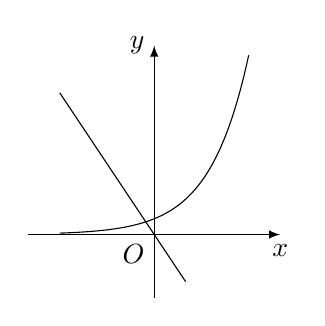
\begin{tikzpicture}[scale = 0.2, >=latex]
    \draw [->] (-8,0) -- (8,0) node [below] {$x$};
    \draw [->] (0,-4) -- (0,12) node [left] {$y$};
    \draw (0,0) node [below left] {$O$};
    \draw [domain = -6:2, samples = 100] plot (\x,{-1.5*\x});
    \draw [domain = -6:6, samples = 100] plot (\x,{1.5^\x});
\end{tikzpicture}}{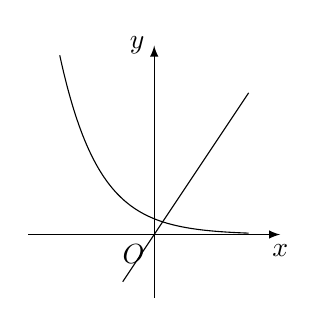
\begin{tikzpicture}[scale = 0.2, >=latex]
    \draw [->] (-8,0) -- (8,0) node [below] {$x$};
    \draw [->] (0,-4) -- (0,12) node [left] {$y$};
    \draw (0,0) node [below left] {$O$};
    \draw [domain = -2:6, samples = 100] plot (\x,{1.5*\x});
    \draw [domain = -6:6, samples = 100] plot (-\x,{1.5^\x});
\end{tikzpicture}}{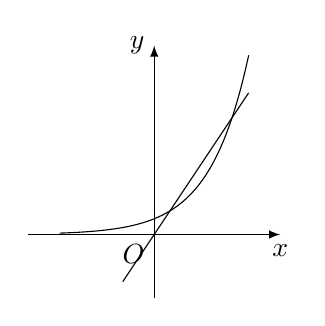
\begin{tikzpicture}[scale = 0.2, >=latex]
    \draw [->] (-8,0) -- (8,0) node [below] {$x$};
    \draw [->] (0,-4) -- (0,12) node [left] {$y$};
    \draw (0,0) node [below left] {$O$};
    \draw [domain = -2:6, samples = 100] plot (\x,{1.5*\x});
    \draw [domain = -6:6, samples = 100] plot (\x,{1.5^\x});
\end{tikzpicture}}{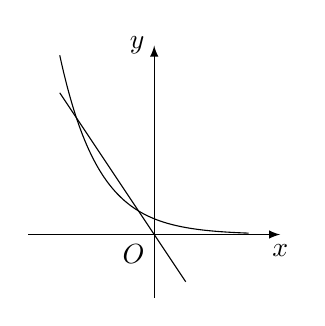
\begin{tikzpicture}[scale = 0.2, >=latex]
    \draw [->] (-8,0) -- (8,0) node [below] {$x$};
    \draw [->] (0,-4) -- (0,12) node [left] {$y$};
    \draw (0,0) node [below left] {$O$};
    \draw [domain = -2:6, samples = 100] plot (-\x,{1.5*\x});
    \draw [domain = -6:6, samples = 100] plot (-\x,{1.5^\x});
\end{tikzpicture}}
\item 下列各式中, 正确的是\bracket{20}.
\fourch{$(\dfrac 12)^{\frac 23}<(\dfrac 15)^{\frac 23}<(\dfrac 12)^{\frac 13}$}{$(\dfrac 12)^{\frac 13}<(\dfrac 12)^{\frac 23}<(\dfrac 15)^{\frac 23}$}{$(\dfrac 15)^{\frac 23}<(\dfrac 12)^{\frac 13}<(\dfrac 12)^{\frac 23}$}{$(\dfrac 15)^{\frac 23}<(\dfrac 12)^{\frac 23}<(\dfrac 12)^{\frac 13}$}
\item 若$f(x)$在$(0,+\infty)$上是减函数, 而$f(a^x)$在$(-\infty ,+\infty)$上是增函数, 则实数$a$的取值范围是\bracket{20}.
\fourch{(0, 1)}{$(0,1)\cup (1,+\infty)$}{$(0,+\infty)$}{$(1,+\infty)$}
\item 函数$y=(\dfrac 12)^{\sqrt {-x^2+x+x}}$为增函数的区间是\bracket{20}.
\fourch{$[-1,\dfrac 12]$}{$(-\infty ,-1]$}{$[2,+\infty)$}{$[\dfrac 12,2]$}
\item 若函数$f(x)=(a^2-1)^x$在$(-\infty ,+\infty)$上是减函数, 则$a$的取值范围是\bracket{20}.
\fourch{$|a|>1$}{$|a|<\sqrt 2$}{$a>\sqrt 2$}{$1<|a|<\sqrt 2$}
\item 若函数$f(x)=a^x-(b+1)$($a>0$且$a\ne 1$)的图像在第一、三、四象限, 则必有\bracket{20}.
\fourch{$0<a<1$且$b>0$}{$0<a<1$且$b<0$}{$a>1$且$b<1$}{$a>1$且$b>0$}
\item 用不等号``$>$''或``$<$''填空:
(1) $1.2^{0.3}$\blank{50}$1$;\\
(2) $0.3^{5.1}$\blank{50}$1$;\\
(3) $(\dfrac 23)^{-\frac 13}$\blank{50}$(\dfrac 32)^{-\frac 13}$;\\
(4) $9^{\frac 13}$\blank{50}$3^{\frac 43}$;\\
(5) $2^{\frac 23}$\blank{50}$3.6^{-\frac 34}$;\\
(6) $0.8^{-2}$\blank{50}$(\dfrac 53)^{-\frac 12}$.
\item 将下列各数从小到大排列:
(1) $0.9^{\frac 34}$, $1.2^{\frac 34}$, 1:\blank{50};\\
(2) $2.5^{\frac 23}$, $(-1.4)^{\frac 23}$, $(-3)^{\frac 13}$:\blank{50};\\
(3) $4.1^{\frac 23}$, $3.8^{-\frac 23}$, $(-1.9)^{\frac 35}$:\blank{50}.
\item 根据条件确定实数$x$的取值范围:\\
(1) $2^x>0.5$:\blank{50};\\
(2) $2^x<1$:\blank{50};\\
(3) $0.2^{2x-1}>\dfrac 1{25}$:\blank{50};\\
(4) $8<(\dfrac 12)^{2x+1}$:\blank{50};\\
(5) $(a^2+a+2)^x>(a^2+a+2)^{1-x}$:\blank{50};\\
(6) $(\dfrac 12)^{x^2+x-2}<1$:\blank{50}.
\item 函数$f(x)=\sqrt {1-6^{x^2+x-2}}$的定义域是\blank{50}.
\item 若函数$f(x)$的定义域是$(0, 1)$, 则函数$f(2^{-x})$的定义域是\blank{50}, $f(3\times 9^x+2\times 3^x)$的定义域是\blank{50}.
\item 函数$y=3^{x^2-3x-2}$为增函数的区间是\blank{50}.
\item 函数$y=(0.2)^{x^2-6x+9}$为增函数的区间是\blank{50}.
\item 函数$y=2^{-|x|}$为增函数的区间是\blank{50}.
\item 函数$y=(\dfrac 12)^{|1+2x|}$为增函数的区间是\blank{50}, 为减函数的区间是\blank{50}.
\item 若函数$y=(\dfrac 12)^{(m^2-1)x}$在$x\in \mathbf{R}$为减函数, 则实数$m$的取值范围是\blank{50}.
\item 若$1\le x\le 2$, 则函数$y=(\dfrac 12)^{x^2-6x+10}$的最大值为\blank{50}.
\item 函数$f(x)=a^{2x}-3a^x+2$($a>0$且$a\ne 1$)的最小值为\blank{50}.
\item 对于函数$y=a^{x^2-4}$($a>0$且$a\ne 1$):\\
(1) 若$0<a<1$, 则$y$有最大值\blank{50};\\
(2) 若$a>1$, 则$y$有最小值\blank{50}.
\item 函数$f(x)=\dfrac 1{3^x-1}$的值域是\blank{50}.
\item 函数$f(x)=\dfrac{3^x}{3^x+1}$的值域是\blank{50}.
\item 若关于$x$的方程$5^x=\dfrac{a+3}{5-a}$有负根, 则实数$a$的取值范围是\blank{50}.
\item 若$0<a<1$, $x>y>1$, 则$a^x$, $x^a$, $a^y$, $y^a$从小到大的排列顺序是\blank{50}.
\item 若$0.9<a<1$, 则$a$, $a^a$, $a^{a^a}$从小到大的排列顺序是\blank{50}.
\item 已知$f(x)=a^{2x^2-3x+1}$, $g(x)=a^{x^2+2x-5}$($a>0$且$a\ne 1$), 确定$x$的取值范围, 使得$f(x)>g(x)$.
\item 若$f(x)=a+\dfrac 1{4^x+1}$是奇函数, 求常数$a$的值.
\item 若$f(x)=x^2(\dfrac 1{a^x-1}+m)$($a>0$且$a\ne 1$)为奇函数, 求常数$m$的值.
\item 已知函数$f(x)=(\dfrac 1{2^x-1}+\dfrac 12)x^3$.\\
(1) 求函数的定义域;\\
(2) 讨论$f(x)$的奇偶性;\\
(3) 求证: $f(x)>0$.
\item 已知$f(x)=\dfrac{a^x-1}{a^x+1}$($a>1$).\\
(1) 判断函数$f(x)$的奇偶性;\\
(2) 求函数$f(x)$的值域;\\
(3) 求证: $f(x)$在区间$(-\infty ,+\infty)$上是增函数.
\item 若$0\le x\le 2$, 求函数$y=4^{x-\frac 12}-3\cdot 2^x+5$的最大值和最小值.
\item 若函数$f(x)=a^{2x}+2a^x-1$($a>0$且$a\ne 1$)在$[-1, 1]$上的最大值为$14$, 求实数$a$的值.
\item 已知函数$f(x)=\dfrac a{a^2-2}(a^x-a^{-x})$($a>0$且$a\ne 1$)在$(-\infty ,+\infty)$上是增函数, 求实数$a$的取值范围.
\item 已知$(a+1)^{-\frac 13}<(3-2a)^{-\frac 13}$, 求实数$a$的取值范围.
\item 已知集合$M=\{x|(x+1)^2\le 1\}$, $P=\{y|y=4^x-a\cdot 2^{x+1}+1,\ x\in M,\ \dfrac 34<a\le 1\}$, 且全集$U=\mathbf{R}$, 求$\complement _U(M\cup P)$.
\item 求方程$x^{\frac 13}+2^x=0$的实根个数.
\item 求关于$x$的方程$a^x+1=-x^2+2x+2a$($a>0$且$a\ne 1$)的实数解的个数.
\item 在同一个平面直角坐标系中, 作出$t(x)=0.5x$与$g(x)=0.2\times 2^x$的图像, 并比较它们的增长情况.
\item 某地区不同身高的未成年男性的体重平均值如下表(身高: $\text{cm}$; 体重: $\text{kg}$):
\begin{center}
    \begin{tabular}{|c|c|c|c|c|c|c|}
        \hline
        身高 & $60$ & $70$ & $80$ & $90$ & $100$ & $110$\\ \hline
        体重 & $6.13$ & $7.90$ & $9.99$ & $12.15$ & $15.02$ & $17.05$\\ \hline
        身高 & $120$ & $130$ & $140$ & $150$ & $160$ & $170$\\ \hline
        体重 & $20.92$ & $26.86$ & $31.11$ & $38.85$ & $47.25$ & $55.05$\\ \hline
    \end{tabular}
\end{center}
为了揭示未成年男性的身高与体重的规律, 甲选择了模型$y=ax^2+bx+c$($a>0$), 乙选择了模型$y=ba^x$($a>1$), 其中$y$表示体重, $x$表示身高.你认为谁选择的模型较好?
\item 用计算器计算并填写下表:
\begin{center}
    \begin{tabular}{|c|c|c|c|c|}
        \hline
        $x$	& $f(x)=x^{\frac 12}$ & $g(x)=x^{0.6}$ & $h(x)=2.1^x$ & $s(x)=2.2^x$ \\ \hline
        $0$ & & & & \\ \hline
        $1$ & & & & \\ \hline
        $2$ & & & & \\ \hline
        $3$ & & & & \\ \hline
        $4$ & & & & \\ \hline
        $5$ & & & & \\ \hline
        $6$ & & & & \\ \hline
        $7$ & & & & \\ \hline
        $8$ & & & & \\ \hline
        $9$ & & & & \\ \hline
        $10$ & & & & \\ \hline
    \end{tabular}
\end{center}
从表中变化的现象可以归纳出哪些函数递增的规律?\\
(1) 幂函数$f(x)$与$g(x)$之间比较得出的规律;
(2) 指数函数$h(x)$与$s(x)$之间比较得出的规律;
(3) 幂函数$f(x)=x^{\frac 12}$与指数函数$h(x)$之间比较得出的规律
\item 求$\log_927$的值.\\
解答在这里  设$\log_927=x$, 根据对数的定义有$9^x=27$.即$3^{2x}=3^3$,
所以$ 2x=3,x=\dfrac 32$, 即$\log_927=\dfrac 32$.
注意  $\log_aN$的定义至关重要, 它始终是解对数问题的首要手段.根据定义, 显然有$\log_a1=0$, $\log_aa=1$, $\log_aa^m=m$, $a^{\log_aN}=N$($a>0$且$a\ne 1$, $N>0$).
学习了换底公式后, 本例还可按以下方法求值:
$\log_927=\dfrac{\log_327}{\log_39}=\dfrac{3\log_33}{2\log_33}=\dfrac 32$, 或$\log_927=\log_{3^2}3^3=\dfrac 32\log_33=\dfrac 32$.
\item 设$3^a=4^b=36$, 求$\dfrac 2a+\dfrac 1b$的值.\\
解答在这里  对已知条件取以6为底的对数, 得
$\dfrac 2a=\log_63$, $\dfrac 1b=\log_62$, 于是$\dfrac 2a+\dfrac 1b=\log_63+\log_62=\log_66=1$.
\item 已知$x=a^{\frac 1{1-\log_ay}}$, $y=a^{\frac 1{1-\log_az}}$求证: $z=a^{\frac 1{1-\log_ax}}$.\\
解答在这里  由$x=a^{\frac 1{1-\log_ay}}$, 得$\log_ax=\dfrac 1{1-\log_ay}$.
同理$\log_ay=\dfrac 1{1-\log_az}$, 代入上式, 消去$\log_ay$,
得$\log_ax=\dfrac 1{1-\dfrac 1{1-\log_az}}=\dfrac{1-\log_az}{-\log_az}$, 即$\log_az=\dfrac 1{1-\log_ax}$, 所以$ z=a^{\frac 1{1-\log_ax}}$.
\item 已知$\log_{12}27=a$, 求$\log_616$.
解答在这里  由已知, 得$a=\log_{12}27=\dfrac{\log_327}{\log_312}=\dfrac 3{1+2\log_32}$, 所以$ \log_32=\dfrac{3-a}{2a}$.
于是$\log_616=\dfrac{\log_316}{\log_36}=\dfrac{4\log_32}{1+\log_32}=\dfrac{4(3-a)}{3+a}$.
\item 若$a=b^2$($b>0$, $b\ne 1$), 则有\bracket{20}.
\fourch{$\log_2a=b$}{$\log_2b=a$}{$\log_ab=2$}{$\log_ba=2$}
\item 若$\log_x\sqrt[7]y=z$, 则$x,y,z$之间满足\bracket{20}.
\fourch{$y^7=x^z$}{$y=x^{7z}$}{$y=7x^z$}{$y=z^{7x}$}
\item $2^{\log_43}$的值等于\bracket{20}.
\fourch{3}{$\sqrt 3$}{$\dfrac{\sqrt 3}3$}{$\dfrac 13$}
\item $\log_ab\cdot \log_3a=5$, 则$b=$\bracket{20}.
\fourch{$a^3$}{$a^5$}{$3^5$}{$5^3$}
\item 若点$P(\lg a,\lg b)$关于$x$轴的对称点的坐标是(0, -1), 则$a$和$b$的值是\bracket{20}.
\fourch{$a=1$, $b=10$}{$a=1$, $b=\dfrac 1{10}$}{$a=10$, $b=1$}{$a=\dfrac 1{10}$, $b=1$}
\item 给出下列四个式子(已知$a>0$, $a\ne 1$, $x>y>0$): \textcircled{1} $\log_ax\cdot \log_ay=\log_a(x+y)$; \textcircled{2} $\log_ax+\log_ay=\log_a(x+y)$; \textcircled{3} $\log_a\dfrac xy=\log_a(x-y)$; \textcircled{4} $\log_a(x-y)=\dfrac{\log_ax}{\log_ay}$.其中正确的有\bracket{20}.
\fourch{$0$个}{$1$个}{$2$个}{$3$个}
\item 若$m>0$, 且$10^x=\lg (10m)+\lg \dfrac 1m$, 则$x$的值为\bracket{20}.
\fourch{$2$}{$1$}{$0$}{$-1$}
\item 若$\lg x=a$, $\lg y=b$, 则$\lg \sqrt x-\lg (\dfrac y{10})^2$的值等于\bracket{20}.
\fourch{$\dfrac 12a-2b-2$}{$\dfrac 12a-2b+2$}{$\dfrac 12a-2b-1$}{$\dfrac 12a-2b+1$}
\item 如果方程$\lg ^2x+(\lg 2+\lg 3)\lg x+\lg 2\cdot \lg 3=0$的两个根为$x_1,x_2$, 那么$x_1\cdot x_2$的值为\bracket{20}.
\fourch{$\lg 2\cdot \lg 3$}{$\lg 2+\lg 3$}{$\dfrac 16$}{$-6$}
\item 若$x=t^{\frac 1{t-1}}$, $y=t^{\frac t{t-1}}$($t>0$, $t\ne 1$), 则$x,y$之间的关系是\bracket{20}.
\fourch{$y^x=x^{\frac 1y}$}{$y^{\frac 1x}=x^y$}{$y^x=x^y$}{$x^x=y^y$}
\item 若$\log_8x=-\dfrac 23$, 则$x=$\blank{50}.
\item 若$\log_x27=\dfrac 34$, 则$x=$\blank{50}.
\item 若$\log_2(\log_5x)=0$, 则$x=$\blank{50}.
\item 若$\log_2(\lg x)=1$, 则$x=$\blank{50}.
\item 若$\log_2[\log_3(\log_5x)]=0$, 则$x=$\blank{50}.
\item 若$\log_2[\log_3(\log_4x)]=\log_3[\log_4(\log_2y)]=\log_4[\log_2(\log_3z)]=0$.则$x+y+z=$\blank{50}.
\item 计算: $2^{\log_4(2-\sqrt 3)^2}+3^{\log_9(2+\sqrt 3)^2}=$\blank{50}.
\item 计算: $2^{1+\dfrac 12\log_25}=$\blank{50}.
\item 计算: $9^{\log_32}=$\blank{50}.
\item 计算: $5^{3-2\log_{25}125}=$\blank{50}.
\item 计算: $\log_{(2-\sqrt 3)}(7+4\sqrt 3)=$\blank{50}.
\item 计算: $\log_6(\sqrt {2+\sqrt 3}+\sqrt {2-\sqrt 3})=$\blank{50}.
\item 计算: $(2+\sqrt 3)^{-1}-\log_{(2+\sqrt 3)}(7+4\sqrt 3)=$\blank{50}.
\item 计算: $-2^2\div (-\dfrac{27}8)^{-\frac 13}-(0.7)^{\lg 1}+\log_3\dfrac 14+\log_312=$\blank{50}.
\item 若$3^x=12^y=8$, 则$\dfrac 1x-\dfrac 1y=$\blank{50}.
\item 若$2^x=7^y=196$, 则$\dfrac 1x+\dfrac 1y=$\blank{50}.
\item 若$2^{6a}=3^{3b}=6^{2c}$, 则$a,b,c$之间的关系式是\blank{50}.
\item 已知正数$a,b$满足$a^2+b^2=7ab$, 求证: $\log_m\dfrac{a+b}3=\dfrac 12(\log_ma+\log_mb)$($m>0$, $m\ne 1$).
\item 已知$\log_a(x^2+1)+\log_a(y^2+4)=\log_a8+\log_ax+\log_ay$($a>0$, $a\ne 1$), 求$\log_8(xy)$的值.
\item 已知只有一个$x$的值满足方程$(1-\lg ^2a)x^2+(1-\lg a)x+2=0$, 求实数$a$的值.
\item 设方程$x^2-\sqrt {10}x+2=0$的两个根为$\alpha ,\beta$, 求$\log_4\dfrac{\alpha ^2-\alpha \beta +\beta ^2}{(\alpha -\beta)^2}$的值.
\item 已知$\lg a$和$\lg b$是关于$x$的方程$x^2-x+m=0$的两个根, 且关于$x$的方程$x^2-(\lg a)x-(1+\lg a)=0$有两个相等的实数根, 求实数$a,b$和$m$的值.
\item 已知函数$f(x)=x^2\lg a+2x+4\lg a$的最大值为3, 求实数$a$的值.
\item 已知函数$f(x)=x^2+(\lg a+2)x+\lg b$, 满足$f(-1)=-2$, 且对一切实数$x$都有$f(x)\ge 2x$, 求实数$a,b$的值.
\item 已知$2\lg \dfrac{x-y}2=\lg x+\lg y$, 求$\dfrac xy$的值.
\item 设$A>B>0$, $A^2+B^2=6AB$, 求证: $\log_a\dfrac{A-B}2=\dfrac 12(\log_aA+\log_aB)$($a>0$且$a\ne 1$).
\item 已知集合$M=\{x,xy,\lg (xy)\}$, $P=\{0,|x|,y\}$, 且满足$M=P$, 求实数$x,y$的值.
\item 已知$12^x=3$, $12^y=2$, 求$8^{\frac{1-2x}{1-x+y}}$的值.
\item 已知不相等的两个正数$a,b$满足$a^{\lg ax}=b^{\lg bx}$, 求$(ab)^{\lg abx}$的值.
\item 已知$x,y,z>0$, 且$\lg x+\lg y+\lg z=0$, 求$x^{\frac 1{\lg y}+\dfrac 1{\lg z}}\cdot y^{\frac 1{\lg z}+\dfrac 1{\lg x}}\cdot z^{\frac 1{\lg x}+\dfrac 1{\lg y}}$的值.
\item 求$y^{\lg 20}\cdot (\dfrac 12)^{\lg 0.7}$的值.
\item 化简$\dfrac{\log_58}{\log_52}$可得\bracket{20}.
\fourch{$\log_54$}{$3\log_52$}{$\log_36$}{$3$}
\item $\dfrac{\log_89}{\log_23}$的值是\bracket{20}.
\fourch{$\dfrac 23$}{$1$}{$\dfrac 32$}{$2$}
\item 若$\log_ab=\log_ba$($a\ne b$, $a\ne 1$, $b\ne 1$), 则$ab$等于\bracket{20}.
\fourch{$1$}{$2$}{$\dfrac 14$}{$4$}
\item $\dfrac 1{\log_{\frac 12}\dfrac 13}+\dfrac 1{\log_{\frac 15}\dfrac 13}$的值所属区间是\bracket{20}.
\fourch{$(-2, -1)$}{$(1, 2)$}{$(-\infty ,-2)$}{$(2, 3)$}
\item 若$\log_37\cdot \log_29\cdot \log_{49}m=\log_4\dfrac 12$, 则$m$的值等于\bracket{20}.
\fourch{$\dfrac 14$}{$\dfrac{\sqrt 2}2$}{$\sqrt 2$}{$4$}
\item 若$x\ne 1$, 则与$\dfrac 1{\log_3x}+\dfrac 1{\log_4x}+\dfrac 1{\log_5x}$相等的式子是\bracket{20}.
\fourch{$\dfrac 1{\log_{60}x}$}{$\dfrac 1{\log_3x\cdot \log_4x\cdot \log_5x}$}{$\dfrac 1{\log_x60}$}{$\dfrac{12}{\log_3 x+\log_4 x+\log_5 x}$}
\item 若$\log_83=p$, $\log_35=q$, 则$\lg 5$(用$p,q$表示)等于\bracket{20}.
\fourch{$\dfrac{3p+q}5$}{$\dfrac{1+3pq}{p+q}$}{$\dfrac{3pq}{1+3pq}$}{$p^2+q^2$}
\item 已知$x,y,z$都是大于$1$的正数, $m>0$, 且$\log_xm=24$, $\log_ym=40$, $\log_{xyz}m=12$, 则$\log_zm$的值为\bracket{20}.
\fourch{$\dfrac 1{60}$}{$60$}{$\dfrac{200}3$}{$\dfrac 3{20}$}
\item 计算: $\log_{64}32=$\blank{50}.
\item 计算: $\log_{\frac 1a}b+\log_ab=$\blank{50}.
\item 计算: $\log_625\cdot \log_53\cdot \log_96=$\blank{50}.
\item 计算: $(\log_25+\log_40.2)(\log_52+\log_{25}0.5)=$\blank{50}.
\item 计算: $\log_2\dfrac 1{25}\cdot \log_3\dfrac 18\cdot \log_5\dfrac 19=$\blank{50}.
\item 计算: $a^{\frac{\log_b(\log_ba)}{\log_ba}}=$\blank{50}.
\item 计算: $a^{\frac{\log_ma-\log_mb}{\log_ma}}=$\blank{50}.
\item 已知$n\in \mathbf{N}^*$, 计算: $(\log_23+\log_49+\log_827+\cdots +\log_{2^n}3^n)\cdot \log_9\sqrt [n]{32}=$\blank{50}.
\item 已知$\log_ax=2$, $\log_bx=1$, $\log_cx=4$, 则$\log_{abc}x=$\blank{50}.
\item 已知$m=\log_25$, 则$2^m-m\lg 2-4=$\blank{50}.
\item 已知$\lg (3x^3)-\lg (3y^3)=9$, 则$\dfrac xy=$\blank{50}.
\item 记$\log_827=m$, 用$m$表示$\log_616$.
\item 已知$\log_37=a$, $\log_34=b$, 求$\log_{12}21$.
\item 已知$\log_23=a$, $\log_35=b$, 求$\log_{15}20$.
\item 已知$a>b>1$, $\log_ab+\log_ba=\dfrac{10}3$, 求$\log_ab-\log_ba$的值.
\item 已知$\log_{2a}a=m$, $\log_{3a}2a=n$, 求证: $2^{1-mn}=3^{n-mn}$.
\item 已知关于$x$的方程$x^2-(\log_2b+\log_a2)x+\log_ab=0$的两根为-1和2, 求实数$a,b$的值.
\item 已知$a^2+b^2=c^2$, 求证$\log_{(c+b)}a+\log_{(c-b)}a=2\log_{(c+b)}a\cdot \log_{(c-b)}a$.
\item 已知正实数$x,y,z$满足$3^x=4^y=6^z$.\\
(1) 求证$\dfrac 1z-\dfrac 1x=\dfrac 1{2y}$;\\
(2) 比较$3x,4y,6z$的大小.
\item 求函数$y=\dfrac{\sqrt {\log_{0.8}x-1}}{2x-1}$的定义域.\\
解答在这里  函数的定义域应满足: $\begin{cases} 2x-1\ne 0, \\ \log_{0.8}x-1\ge 0, \\ x>0, \end{cases}$即$\begin{cases} x\ne \dfrac 12, \\ \log_{0.8}x\ge 1, \\ x>0, \end{cases}$
解得$0<x\le \dfrac 45$且$x\ne \dfrac 12$.故函数的定义域为$\{x|0<x\le \dfrac 45\text{且}x\ne \dfrac 12\}$.
\item 解不等式$\log_{0.2}(x^2+2x-3)>\log_{0.2}(3x+1)$.\\
解答在这里  由已知, 得$\begin{cases} x^2+2x-3>0, \\ 3x+1>0, \\ x^2+2x-3<3x+1, \end{cases}$, 即$\begin{cases} (x+3)(x-1)>0, \\ x^2-x-4<0. \end{cases}$
解得$\begin{cases} x<-3x>1, \\ \dfrac{1-\sqrt {17}}2<x<\dfrac{1+\sqrt {17}}2. \end{cases}\therefore$不等式的解集为$\{x|1<x<\dfrac{1+\sqrt {17}}2\}$.
\item 将$\log_{0.7}0.8$, $\log_{1.1}0.9$, $1.1^{0.9}$由小到大排列.\\
解答在这里  利用对数函数的单调性.
因为$\log_{1.1}0.9<\log_{1.1}1=0$, $\log_{0.7}0.8>\log_{0.7}1=0$, 所以$\log_{1.1}0.9<\log_{0.7}0.8$.
又因为$\log_{0.7}0.8<\log_{0.7}0.7=1$, 由指数函数的单调性知, $1.1^{0.9}>1.1^0=1$, 所以$\log_{0.7}0.8<1.0^{0.9}$.
于是从小到大的排列是$\log_{1.1}0.9<\log_{0.7}0.8<1.1^{0.9}$.
\item 若$0<x<1$, $a>0$, $a\ne 1$, 比较$p=|\log_a(1-x)|$和$q=|\log_a(1+x)|$的大小.\\
解答在这里 解法一  因为$ 0<x<1$, 所以$ 1-x\in (0,1)$, $1+x\in (1,2)$, $1-x^2\in (0,1)$.
若$a>1$, 则$\log_a(1-x)<0$, $\log_a(1+x)>0$,
所以$ q-p=\log_a(1+x)+\log_a(1-x)=\log_a(1-x^2)<0$, 所以$ q<p$;
若$0<a<1$, 则$\log_a(1+x)<0$, $\log_a(1-x)>0$,
所以$ q-p=-\log_a(1+x)-\log_a(1-x)=-\log_a(1-x^2)<0$, 所以$ q<p$.故恒有$p>q$.
解法二  因为$ \dfrac pq=|\dfrac{\log_a(1-x)}{\log_a(1+x)}|=|\log_{(1+x)}(1-x)|=-\log_{(1+x)}(1-x)$
\blank{50}$=\log_{(1+x)}\dfrac 1{1-x}=\log_{(1+x)}\dfrac{1+x}{1-x^2}=1-\log_{(1+x)}(1-x^2),$
且$1+x>1$, $0<1-x^2<1$, 所以$ \log_{(1+x)}(1-x^2)<0$, 于是$\dfrac pq>1$.又$p>0$, $q>0$, 故$p>q$.
解法三  $p^2-q^2=\log_a^2(1-x)-\log_a^2(2+x)=\log_a(1-x^2)\cdot \log_a\dfrac{1-x}{1+x}$,
且$0<1-x^2<1$, $0<\dfrac{1-x}{1+x}<1$, 故无论$a>1$还是$0<a<1$, $\log_a(1-x^2)$和$\log_a\dfrac{1-x}{1+x}$一定同号, 所以$ p^2-q^2>0$.又$p>0$, $q>0$, 所以$ p>q$.
解法四  因为$ p-q=|\log_a(1-x)|-|\log_a(1+x)|=\dfrac 1{|\lg a|}(|\lg (1-x)|-|\lg (1+x)|)$
\blank{50}$=\dfrac 1{|\lg a|}[-\lg (1-x)-\lg (1+x)]=\dfrac 1{|\lg a|}\lg (1-x^2)>0$,
所以$ p>q$.
解法五  因为$ \log_a(1-x)=\log_a\dfrac{1-x^2}{1+x}=\log_a(1-x^2)-\log_a(1+x)$,
且$\log_a(1-x^2)$与$\log_a(1+x)$异号,
所以$ p=|\log_a(1-x)|=|\log_a(1-x^2)-\log_a(1+x)|$
    $=|\log_a(1-x^2)|+|\log_a(1+x)|>|\log_a(1+x)|=q$,
即$p>q$.
\item 求函数$f(x)=\log_{0.2}(x-1)(x+2)$为增函数的区间.\\
解答在这里  函数的定义域为$x<-2$或$x>1$, 且$(x-1)(x+2)=x^2+x-2=(x+\dfrac 12)^2-\dfrac 94$, 它在$(-\infty ,-\dfrac 12)$上为减函数.
所以函数$f(x)$为增函数的区间是$(-\infty ,-2)$.
\item 求函数$f(x)=\log_{\frac 12}(x^2-6x+17)$的值域.\\
解答在这里 令$t=x^2-6x+17=(x-3)^2+8\ge 8$,
所以$ f(x)\le \log_{\frac 12}8=-3$, 即函数的值域是$(-\infty ,-3]$.
\item 已知关于$x$的方程$ax^2-4ax+1=0$的两个实数根$\alpha ,\beta$满足不等式$|\lg \alpha -\lg \beta|\le 1$, 求实数$a$的取值范围.\\
解答在这里  由题设, 应有$\begin{cases} \Delta =4(4a^2-a)\ge 0, \\ \alpha +\beta =4>0, \\ \alpha \beta =\dfrac 1a>0, \\|\lg \dfrac{\alpha }{\beta }|\le 1, \end{cases}$即$\begin{cases} a\le 0a\ge \dfrac 14, \\ \alpha +\beta =4, \\ a>0, \\ -1\le \lg \dfrac{\alpha }{\beta }\le 1. \end{cases}$
由第四式, 得$\dfrac 1{10}\le \dfrac{\alpha }{\beta }\le 10$, 即$\dfrac{11}{10}\le \dfrac{\alpha +\beta }{\beta }\le 11$;
由$\alpha +\beta =4$, 得$\dfrac{11}{10}\le \dfrac 4{\beta }\le 11$, 即$\dfrac 4{11}\le \beta \le \dfrac{40}{11}$.
于是$\dfrac 1a=\alpha \beta =\beta (4-\beta)=-(\beta -2)^2+4$.
如图15所示, $\dfrac 1a\in [\dfrac{160}{121},4]$, 所以$a$的取值范围是$\dfrac 14\le a\le \dfrac{121}{160}$.
\begin{center}
    \begin{tikzpicture}[>=latex]
        \draw [->] (-0.1,0) -- (4.5,0) node [below] {$\beta$};
        \draw [->] (0,-0.1) -- (0,4.5) node [left] {$\dfrac 1a$};
        \draw (0,0) node [below left] {$O$};
        \draw [domain = {4/11}:{40/11}] plot (\x,{4-(\x-2)^2});
        \draw [dashed] (0,{160/121}) -- ({40/11},{160/121}) -- ({40/11},0) (0,4) -- (2,4) -- (2,0) ({4/11},{160/121}) -- ({4/11},0);
        \draw (0,{160/121}) node [left] {$\dfrac{160}{121}$} (0,4) node [left] {$4$};
        \draw ({4/11},0) node [below] {$\dfrac 4{11}$} (2,0) node [below] {$2$} ({40/11},0) node [below] {$\dfrac{40}{11}$};
    \end{tikzpicture}
\end{center}
\item 与函数$y=x$为同一个函数的是\bracket{20}.
\twoch{$y=\sqrt {x^2}$}{$y=\dfrac{x^2}x$}{$y=a^{\log_ax}$($a>0$且$a\ne 1$)}{$y=\log_aa^x$($a>0$且$a\ne 1$)}
\item 若函数$y=f(x)$的反函数是$y=\lg (x-1)+3$($x>1$), 则$f(x)$等于\bracket{20}.
\fourch{$10^{x+3}+1$}{$10^{x-3}-1$}{$10^{x+3}-1$}{$10^{x-3}+1$}
\item 若函数$f(x)=\log_2x+3$($x\ge 1$), 则其反函数$f^{-1}(x)$的定义域是\bracket{20}.
\fourch{$\mathbf{R}$}{$\{x|x\ge 1\}$}{$\{x|0<x<1\}$}{$\{x|x\ge 3\}$}
\item 图中图像所对应的函数可能是\bracket{20}.
\begin{center}
    \begin{tikzpicture}[>=latex]
        \draw [->] (-1,0) -- (3,0) node [below] {$x$};
        \draw [->] (0,-2) -- (0,2) node [left] {$y$};
        \draw (0,0) node [below left] {$O$};
        \draw [domain = -1.4:1.8] plot ({0.5^\x},\x);
        \draw (1,0) node [below] {$1$}; 
    \end{tikzpicture}
\end{center}
\fourch{$y=2^x$}{$y=2^x$的反函数}{$y=2^{-x}$}{$y=2^{-x}$的反函数}
\item 设$f(x)$是定义在$(-\infty ,+\infty)$上的偶函数, 且它在$[0,+\infty)$上是增函数, 记$a=f(-\log_{\sqrt 2}\sqrt 3)$, $b=f(-\log_{\sqrt 3}\sqrt 2)$, $c=f(-2)$, 则$a,b,c$的大小关系是\bracket{20}.
\fourch{$a>b>c$}{$b>c>a$}{$c>a>b$}{$c>b>a$}
\item 下列函数图像中, 不正确的是\bracket{20}.
\begin{center}
    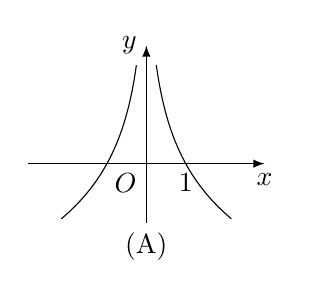
\begin{tikzpicture}[>=latex, scale = 0.5]
        \draw [->] (-3,0) -- (3,0) node [below] {$x$};
        \draw [->] (0,-1.5) -- (0,3) node [left] {$y$};
        \draw (0,0) node [below left] {$O$};
        \draw (1,0) node [below] {$1$};
        \draw [domain = -1.4:2.5] plot ({sqrt((1/3)^\x)},\x);
        \draw [domain = -1.4:2.5] plot ({-sqrt((1/3)^\x)},\x);
        \draw (0,-1.5) node [below] {(A)};
    \end{tikzpicture}
    \begin{tikzpicture}[>=latex, scale = 0.5]
        \draw [->] (-3,0) -- (3,0) node [below] {$x$};
        \draw [->] (0,-1.5) -- (0,3) node [left] {$y$};
        \draw (0,0) node [below left] {$O$};
        \draw (1,0) node [below] {$1$};
        \draw [domain = -0.9:2.5] plot ({-(1/3)^\x},\x);
        \draw (0,-1.5) node [below] {(B)};
    \end{tikzpicture}
    \begin{tikzpicture}[>=latex, scale = 0.5]
        \draw [->] (-3,0) -- (3,0) node [below] {$x$};
        \draw [->] (0,-1.5) -- (0,3) node [left] {$y$};
        \draw (0,0) node [below left] {$O$};
        \draw (1,0) node [below] {$1$};
        \draw [domain = -0.9:2.5] plot ({(1/3)^\x},{abs(\x)});
        \draw (0,-1.5) node [below] {(C)};
    \end{tikzpicture}
    \begin{tikzpicture}[>=latex, scale = 0.5]
        \draw [->] (-3,0) -- (3,0) node [below] {$x$};
        \draw [->] (0,-1.5) -- (0,3) node [left] {$y$};
        \draw (0,0) node [below left] {$O$};
        \draw (1,0) node [below] {$1$};
        \draw [domain = 0.1:2.5] plot (\x,{\x^(-1/3)});
        \draw (0,-1.5) node [below] {(D)};
    \end{tikzpicture}
\end{center}
\fourch{$y=\log_{\frac 13}x^2$}{$y=\log_{\frac 13}(-x)$}{$y=|\log_3x|$}{$y=|x^{-\frac 13}|$}
\item 在同一平面直角坐标系中画出函数$y=x+a$与$y=\log_ax$的图像, 可能是\bracket{20}.
\fourch{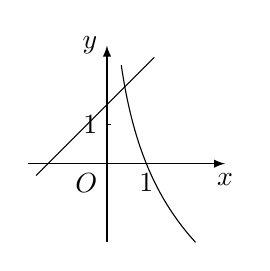
\begin{tikzpicture}[scale = 0.5, >=latex]
    \draw [->] (-2,0) -- (3,0) node [below] {$x$};
    \draw [->] (0,-2) -- (0,3) node [left] {$y$};
    \draw (0,0) node [below left] {$O$};
    \draw (1,0) node [below] {$1$};
    \draw (0.1,1) -- (0,1) node [left] {$1$};
    \draw [domain = -1.8:1.2] plot (\x,{\x+1.5});
    \draw [domain = -2.5:2] plot ({1.5^\x},{-\x}); 
\end{tikzpicture}}
{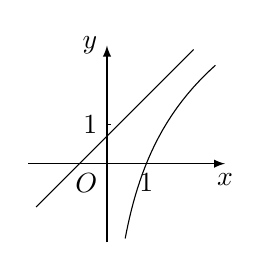
\begin{tikzpicture}[scale = 0.5, >=latex]
    \draw [->] (-2,0) -- (3,0) node [below] {$x$};
    \draw [->] (0,-2) -- (0,3) node [left] {$y$};
    \draw (0,0) node [below left] {$O$};
    \draw (1,0) node [below] {$1$};
    \draw (0.1,1) -- (0,1) node [left] {$1$};
    \draw [domain = -1.8:2.2] plot (\x,{\x+0.7}); 
    \draw [domain = -1.9:2.5] plot ({1.5^\x},{\x}); 
\end{tikzpicture}}
{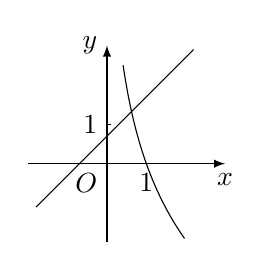
\begin{tikzpicture}[scale = 0.5, >=latex]
    \draw [->] (-2,0) -- (3,0) node [below] {$x$};
    \draw [->] (0,-2) -- (0,3) node [left] {$y$};
    \draw (0,0) node [below left] {$O$};
    \draw (1,0) node [below] {$1$};
    \draw (0.1,1) -- (0,1) node [left] {$1$};
    \draw [domain = -1.8:2.2] plot (\x,{\x+0.7}); 
    \draw [domain = -1.9:2.5] plot ({0.7^\x},{\x}); 
\end{tikzpicture}}
{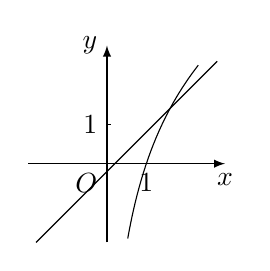
\begin{tikzpicture}[scale = 0.5, >=latex]
    \draw [->] (-2,0) -- (3,0) node [below] {$x$};
    \draw [->] (0,-2) -- (0,3) node [left] {$y$};
    \draw (0,0) node [below left] {$O$};
    \draw (1,0) node [below] {$1$};
    \draw (0.1,1) -- (0,1) node [left] {$1$};
    \draw [domain = -1.8:2.8] plot (\x,{\x-0.2}); 
    \draw [domain = -1.9:2.5] plot ({1.4^\x},{\x}); 
\end{tikzpicture}}
\item 函数$y=f(x)$的图像如图所示, 则$y=\log_{0.7}f(x)$的示意图是\bracket{20}.
\begin{center}
    \begin{tikzpicture}[>=latex]
        \draw [->] (-0.5,0) -- (3,0) node [below] {$x$};
        \draw [->] (0,-0.5) -- (0,3) node [left] {$y$};
        \draw (0,0) node [below left] {$O$};
        \draw (1,0.1) -- (1,0) node [below] {$1$} (2,0.1) -- (2,0) node [below] {$2$} (0.1,1) -- (0,1) node [left] {$1$};
        \draw [dashed] (2,0) -- (2,3);
        \draw [dashed] (1,0) -- (1,1) -- (0,1);
        \draw [domain = 0.3:1.7] plot (\x,{3*(\x-1)^2+1});
    \end{tikzpicture}
\end{center}
\fourch{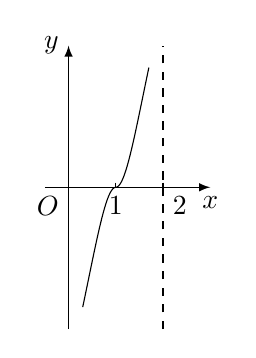
\begin{tikzpicture}[>=latex,scale = 0.6]
    \draw [->] (-0.5,0) -- (3,0) node [below] {$x$};
    \draw [->] (0,-3) -- (0,3) node [left] {$y$};
    \draw (0,0) node [below left] {$O$};
    \draw (1,0.1) -- (1,0) node [below] {$1$} (2,0.1) -- (2,0) node [below right] {$2$};
    \draw [dashed] (2,-3) -- (2,3);
    \draw [domain = 0.3:1] plot (\x,{ln(3*(\x-1)^2+1)/ln(0.7)});
    \draw [domain = 1:1.7] plot (\x,{-ln(3*(\x-1)^2+1)/ln(0.7)});
\end{tikzpicture}}{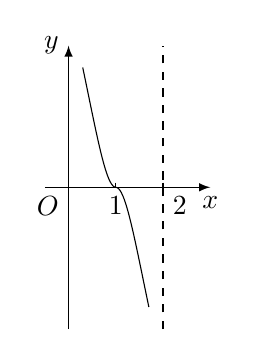
\begin{tikzpicture}[>=latex,scale = 0.6]
    \draw [->] (-0.5,0) -- (3,0) node [below] {$x$};
    \draw [->] (0,-3) -- (0,3) node [left] {$y$};
    \draw (0,0) node [below left] {$O$};
    \draw (1,0.1) -- (1,0) node [below] {$1$} (2,0.1) -- (2,0) node [below right] {$2$};
    \draw [dashed] (2,-3) -- (2,3);
    \draw [domain = 0.3:1] plot (\x,{-ln(3*(\x-1)^2+1)/ln(0.7)});
    \draw [domain = 1:1.7] plot (\x,{ln(3*(\x-1)^2+1)/ln(0.7)});
\end{tikzpicture}}{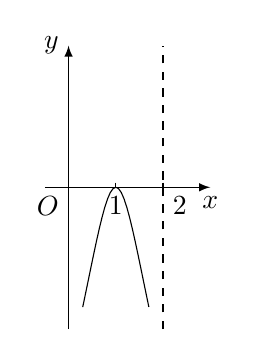
\begin{tikzpicture}[>=latex,scale = 0.6]
    \draw [->] (-0.5,0) -- (3,0) node [below] {$x$};
    \draw [->] (0,-3) -- (0,3) node [left] {$y$};
    \draw (0,0) node [below left] {$O$};
    \draw (1,0.1) -- (1,0) node [below] {$1$} (2,0.1) -- (2,0) node [below right] {$2$};
    \draw [dashed] (2,-3) -- (2,3);
    \draw [domain = 0.3:1.7] plot (\x,{ln(3*(\x-1)^2+1)/ln(0.7)});
\end{tikzpicture}}{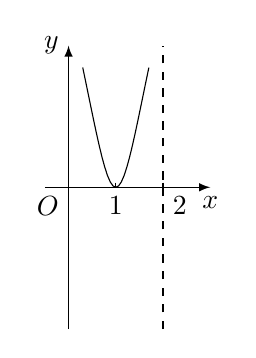
\begin{tikzpicture}[>=latex,scale = 0.6]
    \draw [->] (-0.5,0) -- (3,0) node [below] {$x$};
    \draw [->] (0,-3) -- (0,3) node [left] {$y$};
    \draw (0,0) node [below left] {$O$};
    \draw (1,0.1) -- (1,0) node [below] {$1$} (2,0.1) -- (2,0) node [below right] {$2$};
    \draw [dashed] (2,-3) -- (2,3);
    \draw [domain = 0.3:1.7] plot (\x,{-ln(3*(\x-1)^2+1)/ln(0.7)});
\end{tikzpicture}}
\item 由关系式$\log_xy=3$所确定的函数$y=f(x)$的图像是\bracket{20}.
\fourch{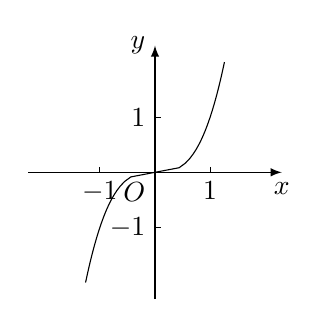
\begin{tikzpicture}[>=latex,scale = 0.7]
    \draw [->] (-2.3,0) -- (2.3,0) node [below] {$x$};
    \draw [->] (0,-2.3) -- (0,2.3) node [left] {$y$};
    \draw (0,0) node [below left] {$O$};
    \draw (1,0.1) -- (1,0) node [below] {$1$} (-1,0.1) -- (-1,0) node [below] {$-1$} (0.1,1) -- (0,1) node [left] {$1$} (0.1,-1) -- (0,-1) node [left] {$-1$};
    \draw [domain = 0:2] plot ({\x^(1/3)},\x);
    \draw [domain = 0:2] plot ({-\x^(1/3)},{-\x});
\end{tikzpicture}}{\begin{tikzpicture}[>=latex,scale = 0.7]
    \draw [->] (-2.3,0) -- (2.3,0) node [below] {$x$};
    \draw [->] (0,-2.3) -- (0,2.3) node [left] {$y$};
    \draw (0,0) node [below left] {$O$};
    \draw (1,0.1) -- (1,0) node [below] {$1$} (-1,0.1) -- (-1,0) node [below] {$-1$} (0.1,1) -- (0,1) node [left] {$1$} (0.1,-1) -- (0,-1) node [left] {$-1$};
    \draw [domain = 0:2] plot ({\x^(1/3)},\x);
    \filldraw [white] (0,0) circle (0.05) (1,1) circle (0.05);
    \draw (0,0) circle (0.05) (1,1) circle (0.05);
\end{tikzpicture}}{\begin{tikzpicture}[>=latex,scale = 0.7]
    \draw [->] (-2.3,0) -- (2.3,0) node [below] {$x$};
    \draw [->] (0,-2.3) -- (0,2.3) node [left] {$y$};
    \draw (0,0) node [below left] {$O$};
    \draw (1,0.1) -- (1,0) node [below] {$1$} (-1,0.1) -- (-1,0) node [below] {$-1$} (0.1,1) -- (0,1) node [left] {$1$} (0.1,-1) -- (0,-1) node [left] {$-1$};
    \draw [domain = 0:2] plot ({\x^(1/3)},\x);
\end{tikzpicture}}{\begin{tikzpicture}[>=latex,scale = 0.7]
    \draw [->] (-2.3,0) -- (2.3,0) node [below] {$x$};
    \draw [->] (0,-2.3) -- (0,2.3) node [left] {$y$};
    \draw (0,0) node [below left] {$O$};
    \draw (1,0.1) -- (1,0) node [below] {$1$} (-1,0.1) -- (-1,0) node [below] {$-1$} (0.1,1) -- (0,1) node [left] {$1$} (0.1,-1) -- (0,-1) node [left] {$-1$};
    \draw [domain = 0:2] plot ({\x^(1/3)},\x);
    \draw [domain = 0:2] plot ({-\x^(1/3)},\x);
\end{tikzpicture}}
\item 若函数$f(x)=\dfrac{1-2^x}{1+2^x}$, 则$f^{-1}(\dfrac 35)$等于\bracket{20}.
\fourch{$3$}{$2$}{$1$}{$-2$}
\item 函数$y=\log_{\frac 13}(x^2-3x+4)$的定义域为\blank{50}.
\item 函数$y=\dfrac{\sqrt {x^2-4}}{\lg (x^2+2x-3)}$的定义域为\blank{50}.
\item 函数$y=\log_{(2x-1)}(32-4^x)$的定义域为\blank{50}.
\item 函数$y=\log_{\frac 13}(x^2-4x+7)$的值域为\blank{50}.
\item 函数$y=\log_{\frac 12}\dfrac 1{x^2-2x+5}$的值域为\blank{50}.
\item 函数$y=\log_{\frac 12}\sqrt {3-2x-x^2}$的值域为\blank{50}.
\item 函数$y=\log_{\frac 13}(x^2-5x+6)$为减函数的区间是\blank{50}.
\item 函数$y=\lg (12-4x-x^2)$为增函数的区间是\blank{50}.
\item 函数$y=-\log_{\frac 12}(-x)$为减函数的区间是\blank{50}.
\item 若函数$y=\log_a(1-x)$在$[0,1)$上是增函数, 则$a$的取值范围是\blank{50}.
\item 函数$y=\log_{\frac 12}^2x-\log_{\frac 12}x+1$为增函数的区间是\blank{50}.
\item 函数$y=(0.2)^{-x}+1$的反函数是\blank{50}.
\item 函数$y=1+\lg (x+2)$($x\ge 8$)的反函数是\blank{50}.
\item 若$f(x)=\dfrac{10^x+1}{10^x-1}$($x>1$), 则$f^{-1}(\dfrac{101}{99})=$\blank{50}.
\item 若$f(x)=\dfrac{\lg x-1}{\lg x+1}$($x>1$且$x\ne \dfrac 1{10}$), 则$f^{-1}(\dfrac 1{10})=$\blank{50}.
\item 若函数$f(x)=a^x-k$的图像过点$(1, 3)$, 其反函数$f^{-1}(x)$的图像过点$(2, 0)$, 则$f(x)$的表达式是\blank{50}.
\item 函数$y=\lg \dfrac{1-x}{1+x}$\bracket{20}.
\twoch{是奇函数, 且在$(-1, 1)$是增函数}{是奇函数, 且在$(-1, 1)$上是减函数}{是偶函数, 且在$(-1, 1)$是增函数}{是偶函数, 且在$(-1, 1)$上是减函数}
\item 函数$f(x)=\ln (\mathrm{e}^x+1)-\dfrac x2$\bracket{20}.
\twoch{是奇函数, 但不是偶函数}{是偶函数, 但不是奇函数}{既是奇函数, 又是偶函数}{没有奇偶性}
\item 求函数$f(x)=\lg (1+x)+\lg (1-x)$ $(-\dfrac 12<x<0)$的反函数.
\item 已知$f(x)=\dfrac{a^x-1}{a^x+1}$($a>1$).\\
(1) 求$f(x)$的值域;\\
(2) 求证: $f(x)$在$R$上是增函数;\\
(3) 求$f(x)$的反函数.
\item 已知$f(\log_ax)=\dfrac{a(x^2-1)}{x(a^2-1)}$($x>0$, $0<a<1$), 求证: 函数$f(x)$在$(-\infty ,+\infty)$上是增函数.
\item 若函数$f(x)=\log_a|x+1|$在$(-1, 0)$上有$f(x)>0$, 则$f(x)$\bracket{20}.
\twoch{在$(-\infty ,0)$上是增函数}{在$(-\infty ,0)$是减函数}{在$(-\infty ,-1)$上是增函数}{在$(-\infty ,-1)$是减函数}
\item 若$0<b<1$, $\log_ab<1$则\bracket{20}.
\fourch{$0<a<b$}{$0<b<a$}{$0<b<a<1$}{$0<a<b$或$a>1$}
\item 若函数$f(x)=|\log_ax|$, 其中$0<a<1$, 则下列各式中成立的是\bracket{20}.
\fourch{$f(\dfrac 13)>f(2)>f(\dfrac 14)$}{$f(\dfrac 14)>f(\dfrac 13)>f(2)$}{$f(2)>f(\dfrac 13)>f(\dfrac 14)$}{$f(\dfrac 14)>f(2)>f(\dfrac 13)$}
\item 若$1<x<2$, 则下列各式正确的是\bracket{20}.
\fourch{$2^x>\log_{\frac 12}x>\sqrt[3]x$}{$2^x>\sqrt[3]x>\log_{\frac 12}x$}{$\sqrt[3]x>2^x>\log_{\frac 12}x$}{$\log_{\frac 12}>x\sqrt[3]x>2^x$}
\item 若函数$f(x)=\log_ax$在$x\in [3,+\infty)$上恒有$|f(x)|>1$, 则实数$a$的取值范围是\bracket{20}.
\twoch{$0<a<\dfrac 13$或$1<a<3$}{$0<a<\dfrac 13$或$a>3$}{$\dfrac 13<a<3$且$a\ne 1$}{$\dfrac 13<a<1$或$a>3$}
\item 若$a>a^2>b>0$, 并记$p=\log_ab$, $q=\log_ba$, $r=\log_a\dfrac ab$, $s=\log_b\dfrac ba$, 则$p,q,r,s$的大小关系是\bracket{20}.
\fourch{$r<q<p<s$}{$r<p<q<s$}{$r<p<s<q$}{$r<q<s<p$}
\item 若$\log_a\dfrac 13>\log_b\dfrac 13>0$, 则$a,b$的关系是\bracket{20}.
\fourch{$1<b<a$}{$1<a<b$}{$0<a<b<1$}{$0<b<a<1$}
\item 将下列各数按从小到大排列: $a=|\log_{\frac 13}\dfrac 14|$, $b=|\log_{\frac 12}\dfrac 32|$, $c=|\log_25|$:\blank{50}.
\item 将下列各数按从小到大排列: $\log_{0.1}0.4$, $\log_{\frac 12}0.4$, $\log_30.4$, $\lg 0.4$:\blank{50}.
\item 将下列各数按从小到大排列: $\dfrac 32$, $\log_23$:\blank{50}.
\item 将下列各数按从小到大排列: $\dfrac 2{\lg 2}$, $\dfrac 3{\lg 3}$, $\dfrac 5{\lg 5}$:\blank{50}.
\item 将下列各数按从小到大排列: $\lg ^2x$, $\lg x^2$, $\lg (\lg x)$, 其中$1<x<10$:\blank{50}.
\item 若$\log_a\dfrac 45<1$($a>0$, $a\ne 1$), 则$a$的取值范围是\blank{50}.
\item 若$0<a<1$, $0<b<1$, 且$a^{\log_b(x-3)}<1$, 则$x$的取值范围是\blank{50}.
\item 求函数$y=(\log_{\frac 14}x)^2-\log_{\frac 14}x^2+5$($2\le x\le 4$)的值域.
\item 若$-3\le \log_{\frac 12}x\le -\dfrac 12$, 求$y=(\log_2\dfrac x2)(\log_2\dfrac x4)$的最大(小)值及其相应的$x$值,
\item 已知$a,b$是两个不相等的正数, 且$\log_m\dfrac xa\cdot \log_m\dfrac xb$的最小值是$-\dfrac 14$($m>0$且$m\ne 1$), 求$m$的值.
\item 已知实数$x,y$满足$(\log_4y)^2=\log_{\frac 12}x$, 求$u=\dfrac xy$的最大值及其相应的$x,y$的值.
\item 已知抛物线$y=x^2\log_2a+2x\log_a2+8$位于$x$轴的上方, 求实数$a$的取值范围.
\item 已知函数$f(x)=(\log_ab)x^2+2(\log_ba)x+8$的图像在$x$轴的上方, 求$a,b$的取值范围.
\item 若只有一个$x$的值满足方程$(1-\lg ^2a)x^2+(1-\lg a)x+2=0$, 求实数$a$的值.
\item 若关于$x$的方程$x^2+2(\log_3a+1)x-\log_9a=0$有两个相等实根, 求实数$a$的值.
\item 若二次函数$f(x)=(\lg a)x^2+2x+4\lg a$有最小值$-3$, 求实数$a$的值.
\item 已知$f(x)=\log_a|\log_ax|$($0<a<1$).\\
(1) 解不等式: $f(x)>0$;\\
(2) 判断$f(x)$在$(1,+\infty)$上的单调性, 并证明之.
\item 实数$a$为何值时, 函数$f(x)=2^x-2^{-x}\lg a$为奇函数?
\item 已知函数$f(x)=\sqrt {\log_ax-1}$($a>0$且$a\ne 1$).\\
(1) 求$f(x)$的定义域;\\
(2) 当$a>1$时, 求证: $f(x)$在$[a,+\infty)$上是增函数.
\item 已知函数$f(x)=1+\log_x3$, $g(x)=2\log_x2$($x>0$, 且$x\ne 1$), 比较$f(x)$与$g(x)$的大小.
\item 当$a>1$时, 比较$\log_ba$与$\log_{2b}a$的大小.
\item 已知$\log_ma>\log_na$($a>1$), 讨论$m$与$n$的大小关系.
\item 已知$\log_{1+a}(1-a)<1$, 求实数$a$的取值范围.
\item 已知$|\lg (1-a)|>|\lg (1+a)|$, 求实数$a$的取值范围.
\item 已知函数$f(x)=\log_{\frac 12}(x^2-2x)$.\\
(1) 求它的单调区间;\\
(2) 求$f(x)$为增函数时的反函数.
\item 已知函数$f(x)=\log_a\dfrac{x+b}{x-b}$($a>0$, $b>0$且$a\ne 1$).\\
(1) 求$f(x)$的定义域;\\
(2) 讨论$f(x)$的奇偶性;\\
(3) 讨论$f(x)$的单调性;\\
(4) 求$f(x)$的反函数$f^{-1}(x)$.
\item 已知函数$f(x)=\lg \dfrac{x+1}{x-1}+\lg (x-1)+\lg (a-x)$($a>1$).\\
(1) 是否存在一个实数$a$使得函数$y=f(x)$的图像关于某一条垂直于$x$轴的直线对称? 若存在, 求出这个实数$a$; 若不存在, 说明理由;\\
(2) 当$f(x)$的最大值为2时, 求实数$a$的值.
\item 解方程$9^{2x-1}=4^x$.\\
解答在这里  由题意.可得$(\dfrac 92)^{2x}=9$, 所以$ 2x=\log_{\frac 92}9$, 故$x=\dfrac 12\log_{\frac 92}9$.
\item 解方程$(\dfrac 1{27})^x=9^{1-x}$.\\
解答在这里  方程即为$3^{-3x}=3^{2-2x}$, 所以$ -3x=2-2x$, 故$x=-2$.
\item 解方程$9^x-2\cdot 3^{x+1}-27=0$.\\
解答在这里  令$y=3^x>0$, 则原方程可化为$y^2-6y-27=0$.
由此得$y=9$(另一解$y=-3$舍去).从而由$3^x=9$, 解得$x=2$.
\item 解方程$9^x+4^x=\dfrac 52\times 6^x$.\\
解答在这里 方程即为$2\times 3^{2x}-5\times 3^x\times 2^x+2\times 2^{2x}=0$, 即$2(\dfrac 32)^{2x}-5\times (\dfrac 32)^x+2=0$.
令$y=(\dfrac 32)^x$, 方程又化为$2y^2-5y+2=0$, 解得$y_1=2$, $y_2=\dfrac 12$,
于是便可得$x_1=\log_{\frac 23}2$, $x_2=\log_{\frac 23}2$.
\item 解方程$\log_3(3^x-1)\cdot \log_3(3^{x-1}-\dfrac 13)=2$.\\
解答在这里  方程即为$\log_3(3^x-1)\cdot \log_3[\dfrac 13(3^x-1)]=2$.
令$t=\log_3(3^x-1)$, 则方程可化为$t(t-1)-2=0$, 解得$t_1=2$, $t_2=-1$.
于是由$\log_3(3^x-1)=2$, 得$3^x=10$, 所以$ x=\log_310$.
由$\log_3(3^x-1)=-1$, 得$3^x=\dfrac 43$, 所以$ x=\log_3\dfrac 43$.
故原方程的解为$x_1=\log_310$, $x_2=\log_3\dfrac 43$.
\item 已知关于$x$的方程$\lg (kx)=2\lg (x+1)$有且只有一个实数解, 求实数$k$的取值范围.\\
解答在这里  显然, $x$需满足
$\begin{cases} kx>0, \\ x+1>0, \\ (x+1)^2=kx, \end{cases}$即$\begin{cases} x>-1, \\ x^2+(2-k)x+1=0. \end{cases}$.
(1) 若上述方程有两个相等实根, 则必有$\Delta =0$, 即$(2-k)^2-4=0$,
所以$ k=0$或$k=4$.
若$k=0$, 得实根$x=-1$应舍去; 若$k=4$, 得实根$x=1$符合题意.
(2) 若上述方程有两个不等实根$x_1,x_2$,
则必有$x_1>-1$, $x_2\le -1$.
考虑函数$f(x)=x^2+(2-k)x+1$.
\begin{center}
    \begin{tikzpicture}
        \draw [->] (-2,0) -- (2,0) node [below] {$x$};
        \draw [->] (0,-2) -- (0,2) node [left] {$y$};
        \draw (0,0) node [below right] {$O$};
        \draw [dashed] (-1,-2) -- (-1,0) node [below right] {$-1$} -- (-1,2);
        \draw [domain = -1.5:1.6] plot (\x,{(\x-0.1)^2-1.5});
    \end{tikzpicture}
\end{center}
如图, 只需$f(-1)\le 0$, 即$1+(2-k)(-1)+1\le 0$,
所以$ k\le 0$. 由(1)知, $k=0$不合题意.
综上所述, 实数$k$的取值范围是$k=4$或$k<0$.
\item 若$2^{2x}+4=5\times 2^x$, 则$x^2+1$等于\bracket{20}.
\fourch{$1$}{$5$}{$5$或$1$}{$3$或$2$}
\item 方程$2^{|x+1|}=3$的解集是\bracket{20}.
\fourch{$\{\log_{\frac 12}\dfrac 23\}$}{$\{\log_2\dfrac 23\}$}{$\{\log_2\dfrac 32,\log_2\dfrac 16\}$}{$\{\log_2\dfrac 13,-\log_{\frac 12}6\}$}
\item 方程$2x^2+2^x-3=0$的实数根有\bracket{20}.
\fourch{$0$个}{$1$个}{$2$个}{无数个}
\item 满足$(x-2)^{5-|x|}=1$的实数根存\bracket{20}.
\fourch{$4$个}{$3$个}{$2$个}{无数个}
\item 方程$6\cdot 7^{|x|}-7^{-x}=1$的解集是\bracket{20}.
\fourch{$\{\log_7\dfrac 12\}$}{$\{\log_75\}$}{$\{\log_7\dfrac 12,\log_75\}$}{$\varnothing$}
\item 若对于任意实数$p$, 函数$y=(p-1)2^x-\dfrac p2$的图像恒过一定点, 则这个点的坐标是\bracket{20}.
\fourch{$(1,-\dfrac 12)$}{$(0, -1)$}{$(-1,-\dfrac 12)$}{$(-2,-\dfrac 14)$}
\item 方程$2^{2x+1}-33\cdot 2^{x-2}+1=0$的解是\bracket{20}.
\fourch{$\{-2,-3\}$}{$\{2,-3\}$}{$\{2,3\}$}{$\{-2,3\}$}
\item 方程$3^{x^2}=(3^x)^2$的解为\blank{50}.
\item 方程$3^x=2^x$的解为\blank{50}.
\item 方程$\dfrac{3^{x^2+1}}{3^{x-1}}=81$的解为\blank{50}.
\item 方程$5^{x-1}\cdot 10^{3x}=8^x$的解为\blank{50}.
\item 方程$2^{x-1}=3^{2x}$的解为\blank{50}.
\item 方程$2\cdot 4^x-7\cdot 2^x+3=0$的解为\blank{50}.
\item 方程$9^x-3^{x+2}-10=0$的解为\blank{50}.
\item 方程$3^{x+1}-3^{-x}=2$的解为\blank{50}.
\item 已知$a>0$且$a\ne 1$, 则方程$a(a^x+1)=a^{-x}+1$的解为\blank{50}.
\item 解方程: $3\times 16^x+36^x=2\times 81^x$.
\item 解方程: $(\sqrt {5+2\sqrt 6})^x+(\sqrt {5-2\sqrt 6})^x=10$.
\item 解方程: $\sqrt[x]9-\sqrt[x]6=\sqrt[x]4$.
\item 解方程: $4^{x+\sqrt {x^2-2}}-5\times 2^{x-1+\sqrt {x^2-2}}=6$.
\item 已知关于$x$的方程$2a^{2x-2}-7a^{x-1}+3=0$有一个根是$2$, 求实数$a$的值, 并求方程其余的根.
\item 解关于$x$的方程$\dfrac{a^x-a^{-x}}{a^x+a^{-x}}=b$(实数$a>0$, $a\ne 1$, $b\in \mathbf{R}$).
\item 若关于$x$的指数方程$9^x+(a+4)3^x+4=0$有实数解, 试求实数$a$的取值范围.
\item 若关于$x$的方程$2a\cdot 3^{-|x-1|}-3^{-2|x-1|}-2a-1=0$有实数解, 求实数$a$的取值范围.
\item 方程$\lg (x-1)^2=2$的解集是\bracket{20}.
\fourch{$\{11\}$}{$\{-9\}$}{$\{11,-9\}$}{$\{-11,9\}$}
\item 关于$x$的方程$\log_ax^2=\log_a(\sqrt {a+1}-\sqrt a)-\log_a(\sqrt {a+1}+\sqrt a)$($a>0$且$a\ne 1$)的解为\bracket{20}.
\fourch{$\sqrt {a+1}+\sqrt a$}{$\sqrt {a+1}-\sqrt a$}{$\pm (\sqrt {a+1}+\sqrt a)$}{$\pm (\sqrt {a+1}-\sqrt a)$}
\item 若$f(x)=1+\lg x$, $g(x)=x^2$, 则使$2f[g(x)]=g[f(x)]$成立的$x$值等于\bracket{20}.
\fourch{$10^{1+\sqrt 2}$或$10^{1-\sqrt 2}$}{$1+\sqrt 2$或$1-\sqrt 2$}{$10^{1+\sqrt 3}$或$10^{1-\sqrt 3}$}{$1+\sqrt 3$或$1-\sqrt 3$}
\item 方程$\log_5(x-8)^2=2+\log_5(x-2)$的解是\bracket{20}.
\fourch{3或$\dfrac 12$}{$\dfrac 12$}{$3$或$38$}{$2$}
\item 方程$\sqrt {\lg x-4}=4-\lg x$的解集是\bracket{20}.
\fourch{$\{100\}$}{$\{1000\}$}{$\{10000\}$}{$\{\dfrac 1{10000}\}$}
\item 方程$\log_2(x-1)-\log_4(x+5)=0$的解为\blank{50}.
\item 方程$\log_4(2-x)=\log_2(x-1)-1$的解为\blank{50}.
\item 方程$\log_x(x^2-x)=\log_x2$的解为\blank{50}.
\item 方程$\log_{(16-3x)}(x-2)=\log_82\sqrt 2$的解为\blank{50}.
\item 方程$\lg|2x-3|-\lg|3x-2|=0$的解为\blank{50}.
\item 方程$\lg ^2x+\lg x^3+2=0$的解为\blank{50}.
\item 方程$\lg ^2x+\lg x^2-3=0$的解为\blank{50}.
\item 方程$(\log_4x)^2-\dfrac 12|\log_2x|-2=0$的解为\blank{50}.
\item 已知方程$\ln ^2x-\ln x^2-2=0$的两个根为$\alpha ,\beta$, 求$\log_{\alpha }\beta +\log_{\beta }\alpha$的值.
\item 已知集合$A=\{x|x^2-ax+a^2-19=0\}$, $B=\{x|\log_2(x^2-5x+8)=1\}$, $C=\{x|x^2+2x-8=0\}$满足$A\cap B\ne \varnothing$, $A\cap C\ne \varnothing$, 求实数$a$的值.
\item 已知$f(x)=\log_a(a^x-1)$($a>0$, $a\ne 1$), 解方程$f(2x)=f^{-1}(x)$.
\item 解方程$\log_{\frac 12}(9^{x-1}-5)=\log_{\frac 12}(3^{x-1}-2)-2$.
\item 解方程$\log_{0.5x}2-\log_{0.5x^3}x^2=\log_{0.5x^3}4$.
\item 解方程$(\sqrt x)^{\log_5x-1}=5$.
\item 解方程$10^{\lg ^2x}+x^{\lg x}=20$.
\item 解方程$|\log_2x|=|\log_2(2x^2)|-2$.
\item 解方程组$\begin{cases} \log_yx-3\log_xy=2, \\ (2^x)^y=(\dfrac 12)^{-16}. \end{cases}$.
\item 解关于$x$的方程: $\lg (x+a)+1=\lg (ax-1)$.
\item 解关于$x$的方程: $\lg (ax-1)-\lg (x-3)=1$.
\item 解关于$x$的方程: $2\lg x-\lg (x-1)=\lg a$.
\item 已知函数$f(x)=a^{x-\dfrac 12}$满足$f(\lg a)=\sqrt {10}$, 求实数$a$的值.
\item 已知函数$f(x)=x^2-x+k$满足$\log_2f(a)=2$, $f(\log_2a)=k$($a>0$且$a\ne 1$), 求$f(\log_2x)$在什么区间上是减函数, 并求出$a$与$k$的值.
\item 若关于$x$的方程$\lg 2x\cdot \lg 3x=-a^2$有两个相异实根, 求实数$a$的取值范围, 并求此方程两根之积.
\item 若关于$x$的方程$(\lg ax)(\lg ax^2)=4$所有的解都大于$1$, 求实数$a$的取值范围.
\item 若关于$x$的方程$\lg (ax)\cdot \lg (ax^2)=4$有两个小于$1$的正根$\alpha ,\beta$, 且满足$|\lg \alpha -\lg \beta|\le 2\sqrt 3$, 求实数$a$的取值范围.
\item 已知函数$f(x)=x^2\lg a+2x+4\lg a$的最大值是$3$, 求实数$a$的值.
\item 若关于$x$的方程$\log_2x+1=2\log_2(x-a)$恰有一个实数解, 求实数$a$的取值范围.
\item 已知函数$f(x)=\log_a(a-ka^x)$($a>0$, $a\ne 1$, $k\in \mathbf{R}$).
(1) 当$0<a<1$, 且$1\le x$时, $f(x)$都有意义, 求实数$k$的取值范围;\\
(2) 当$a>1$时, $f(x)$的反函数就是它自身, 求$k$的值;\\
(3) 在(2)的条件下, 求$f^{-1}(x^2-2)=f(x)$的解.
\item 已知$A=\{0,1\}$, $B=\{x|x\subseteq A\}$, 问: $A$与$B$是什么关系, 并用列举法写出$B$.
\item 已知$f(x)=x^2+ax+b$($a,b$均为实数), 集合$A=\{x|x=f(x) ,x\in \mathbf{R}\}=\{-1,3\}$, $B=\{x|x=f[f(x)],x\in \mathbf{R}\}$, 用列举法求集合.
\item 已知实数集$\mathbf{R}$的子集$P$满足两个条件: \textcircled{1} $1\notin P$; \textcircled{2} 若实数$a\in P$, 则$\dfrac 1{1-a}\in P$. 求证:\\
(1) 若$2\in P$, 则$P$中必含有其他两个数, 并求出这两个数;\\
(2) 集合$P$不可能是单元素集.
\item 已知集合$A,B,C$满足$A\cap B=A$, $B\cap C=B$, 求证: $A\subseteq C$.
\item 已知集合$A=\{x|x=a^2+1,\ a\in \mathbf{N}\}$, $B=\{y|y=b^2-4b+5,\ b\in \mathbf{N}\}$, 求证: $A\subset B$.
\item 已知集合$A=\{x|x=12a+8b,\ a,b\in \mathbf{Z}\}$, $B=\{x|x=20c+16d,\ c,d\in \mathbf{Z}\}$, 求证: $A=B$.
\item 某班学生期中考试数学得优秀的有$18$人, 物理得优秀的有$14$人, 其中数学、物理两科中至少有一科得优秀的有$22$人, 求两科都得优秀的学生人数.
\item 由某班学生组成的篮球队、排球队、乒乓球队分别有$14, 15, 13$名队员.已知同时参加这三个队的有$3$人, 既参加篮球队又参加排球队的有$5$人, 仅参加乒乓球队的有$4$人, 仅参加排球队的有$5$人, 问: 仅参加篮球队的有几人.
\item 某地区先后举行中学生数、理、化三科竞赛, 参加竞赛的学生人数依次是$807$人、$739$人、$437$人, 其中参加数学、物理两科竞赛的有$513$人, 参加物理、化学竞赛的有$267$人, 参加数学、化学竞赛的有$371$人, 三科竞赛都参加的有$213$人, 求参加竞赛的学生总人数.
\item 已知集合$A=\{(x,y)|\dfrac{y-3}{x-2}=a+1\}$, $B=\{(x,y)|(a^2-1)x+(a-1)y=15\}$满足$A\cap B=\varnothing$, 求实数$a$的值.
\item 已知集合$A=\{x|x^2-(a+1)^2x+2a^3+2a\le 0,x\in \mathbf{R}\}$, $B=\{x|x^2-3(a+1)x+6a+2\le 0,x\in \mathbf{R}\}$满足$A\subseteq B$, 求实数$a$的取值范围.
\item 从集合$A=\{1,2,3\}$到集合$M=\{0,1\}$可以建立几个不同的映射?
\item 从集合$P=\{1,2\}$到集合$Q=\{3,4,5\}$可以建立几个不同的映射?
\item 若函数$f(x)$的定义域为$\mathbf{R}^+$, 且满足$f(xy)=f(x)+f(y)$, $f(8)=3$, 求$f(\sqrt 2)$的值.
\item 若函数$f(x)$的定义域为$\mathbf{R}$, 且满足$f(x)+2f(-x)=-x^3+6x^2-3x+3$, 求$f(0)$的值, 并求$f(x)$的表达式.
\item 已知$f(x+y)=f(x)+f(y)$对于任何实数$x,y$都成立.\\
(1) 求证: $f(2x)=2f(x)$;\\
(2) 求$f(0)$的值;\\
(3) 求证: $f(x)$为奇函数.
\item 已知函数$f(x)$对任何实数$x,y$满足$f(x+y)+f(x-y)=2f(x)f(y)$, 且$f(0)\ne 0$, 求证: $f(x)$是偶函数.
\item 已知函数$f(x)$($x\ne 0$)满足$f(xy)=f(x)+f(y)$.
(1) 求证: $f(1)=f(-1)=0$;\\
(2) 求证: $f(x)$为偶函数;\\
(3) 若$f(x)$在$(0,+\infty)$上是增函数, 解不等式$f(x)+f(x-\dfrac 12)\le 0$.
\item 已知函数$f(x)$对一切实数$x,y$满足$f(0)\ne 0$, $f(x+y)=f(x)\cdot f(y)$, 且当$x<0$时, $f(x)>1$.求证:
(1)当$x>0$时, $0<f(x)<1$.
(2)$f(x)$在$x\in \mathbf{R}$上是减函数.
\item (1)求函数$y=2x+\sqrt {1-2x}$的最大值.
(2)求函数$y=2x+\sqrt {1-x^2}$的值域.
(3)求函数$y=\dfrac{\sqrt {x+1}}{x+2}$的值域.
\item 求函数$g(t)=(t+3)(1+|t-1|)$的值域, 其中实数$t$的取值范围是使函数$f(x)=x^2-4tx+2t+30$对任一$x\in \mathbf{R}$都取非负值.
\item 已知函数$f(x)$的定义域是[0, 1], 求函数$f(x+m)+f(x-m)$的定义域(其中$m>0$).
\item 已知集合$A=\{x|x^2-5x+4\le 0\}$, $B=\{x|x^2-2ax+a+2\le 0\}$满足$A\supseteq B\ne \varnothing$, 求实数$a$的取值范围.
\item 已知函数$f(x)=x^2-2mx+m+6$.\\
(1) 若对任意实数$x$都有$f(x)>0$, 求实数$m$的取值范围;\\
(2) 若实数$\alpha ,\beta$满足$f(\alpha)=f(\beta)=0$, 求$\alpha ^2+\beta ^2$的最小值.
\item 已知函数$f(x)=x^2-2kx+2$在$x\ge -1$时恒有$f(x)\ge k$, 求实数$k$的取值范围.
\item 已知$f(x)=-9x^2-6ax+2a-a^2$在$-\dfrac 13\le x\le \dfrac 13$内有最大值$-3$, 求实数$a$的值.
\item 已知$y=f(x)$在其定义域上是增函数, 求证: $y=f(x)$的反函数$y=f^{-1}(x)$在其定义域上也是增函数.
\item 已知函数$f(x)=x^3+x+1$($x\in \mathbf{R}$), 求证:\\
(1) $f(x)$是$\mathbf{R}$上的增函数;\\
(2) 方程$x^3+x+1=0$只有一个实数解.
\item 已知函数$f(x)=\dfrac x{1+x^2}$($x\in \mathbf{R}$).\\
(1) 求$f(x)$的值域;\\
(2) 讨论$f(x)$的单调性.
\item 若二次函数$f(x)=ax^2+bx+c$满足$f(x_1)=f(x_2)$, ($x_1\ne x_2$)求证: 直线$x=\dfrac{x_1+x_2}2$是该二次函数图像的对称轴.
\item 若对于任何实数$x$, 函数$y=f(x)$始终满足$f(a+x)=f(a-x)$, 求证: 函数$y=f(x)$的图像关于直线$x=a$对称.
\item 已知函数$f(x)$满足$f(x+2)=f(2-x)$($x\in \mathbf{R}$), 且$f(x)$的图像与$x$轴有15个不同的交点, 求方程$f(x)=0$的所有解的和.
\item 已知函数$f(2x+1)$是偶函数, 求函数$f(2x)$的图像的对称轴.
\item 求函数$y=\dfrac{3x-1}{x+2}$($x\ne -2$)的图像的对称点.
\item 已知函数$f(x)$满足$f(x)+f(2-x)+2=0$($x\in \mathbf{R}$), 求$f(x)$的图像的对称中心.
\item 已知函数$f(x)=\log_3(x^2-4mx+4m^2+m+\dfrac 1{m-1})$, 集合$M=\{m|m>1,m\in \mathbf{R}\}$.\\
(1) 求证: 当$m\in M$时, $f(x)$的定义域为$x\in \mathbf{R}$; 反之, 若$f(x)$对一切实数$x$都有意义, 则$m\in M$;\\
(2) 当$m\in M$时, 求$f(x)$的最小值;\\
(3) 求证: 对每一个$m\in M$, $f(x)$的最小值都不小于1.
\item 已知函数$f(x)=\dfrac{4^x}{4^x+2}$, 求$f(\dfrac 1{101})+f(\dfrac 2{101})+\cdots +f(\dfrac{100}{101})$的值.
\item 已知函数$f(x)=1+\log_x5$, $g(x)=\log_{x^2}9+\log_{x^2}8$, 比较$f(x)$与$g(x)$的大小.
\item 求方程$x^2-4|x|-\log_2x-5=0$的实数解的个数.
\item 求使方程$|x^2-2x+1+a|=a^2-6$恰有两相异实数解时$a$的取值范围.
\item 已知$f(x)$在$(-\infty ,+\infty)$上有单调性, 且满足$f(1)=2$和$f(x+y)=f(x)+f(y)$.\\
(1) 求证: $f(x)$为奇函数;\\
(2) 若$f(x)$满足$f(k\log_2t)+f(\log_2t-\log_2^2t-2)<0$, 求实数$k$的取值范围.
\item 已知函数$f(x)$在定义域$x\in \mathbf{R}^+$上是增函数, 且满足$f(x\cdot y)=f(x)+f(y)$($x,y\in \mathbf{R}^+$).\\
(1) 求$f(x)$在$(1,+\infty)$上的值域;\\
(2) 若$f(2)=1$, $f(x)$图像上三点$A,B,C$的横坐标分别为$a,a+2,a+4$($a>0$), 且$\triangle ABC$的面积小于$1$, 求实数$a$的取值范围.
\item 求关于$x$的方程$9^{-|x-2|}-4\cdot 3^{-|x-2|}-a=0$有实根的条件.
\item 解方程$|\log_2x|=|\log_22x^2|-2$.
\item 分别求实数$a$的取值范围, 使关于$x$的方程$\log_{(x+a)}2x=2$有唯一解、两解、无解.
\item 分别求实数$a$的范围, 使关于$x$的方程$1+\dfrac{\log_2(2\lg a-x)}{\log_2x}=2\log_x2$有两解、一解.


\end{enumerate}
\end{document}